\documentclass{noithesis}
\usepackage{amsmath}
\usepackage{amsthm}
\usepackage{array}
\usepackage{ctex}
\usepackage{graphicx}
\usepackage{subfigure}
\usepackage{amsmath}
\usepackage{amssymb}
\usepackage{tabularx}
\usepackage{multirow}
\usepackage{hyperref}
\hypersetup{
	colorlinks=true,
	linkcolor=black,
	filecolor=black,      
	urlcolor=black,
	citecolor=black,
}
\usepackage{ulem}

\bibliographystyle{plain}
\begin{document}
\setcounter{page}{1}
	\newtheorem{definition}{\hspace{2em}定义}[section]
	\newtheorem{theorem}{\hspace{2em}定理}[section]
	\newtheorem{lemma}{\hspace{2em}引理}[section]
	\newtheorem{problem}{\hspace{2em}例题}[section]
	\title{浅谈棋盘模型在计数问题中的应用}
	\author{长郡中学\ 彭思进}
	\date{}
	
	\maketitle
	
	\def \bangle{ \atopwithdelims \langle \rangle}
	
\section{前言}
	
	棋盘是一类重要的组合模型,其基本问题为计算在一个棋盘上放置若干个车使得任意两个车无法互相攻击的方案数。其简洁直观的特点使得其在大量计数问题中得到了应用,但在信息学竞赛中大部分题目仅考察了最基本的禁区排列问题。本文将在禁区排列问题的基础上介绍通过棋盘理论可以求解的其他计数问题。
	
	本文第 2,3 节对本文所使用的符号约定与基本元素的定义进行阐述;第 4 节介绍关于棋盘的三个基础定理;第 5 节讨论了两个经典的禁区排列问题;第 6 节讨论了一类特殊棋盘—— Ferrers 棋盘的棋盘多项式求解以及其应用与变式;第 7,8,9 节则分别从排列的降低、逆序对数、环数三个方面分别介绍棋盘模型在排列计数问题中的应用。
	
\section{约定}
	
	假定读者已经掌握多项式的基本运算与基本的组合计数知识。
	
	对于一个多项式或幂级数 $f(x)$,约定 $[x^k]f(x)$ 为 $f(x)$ 的 $x^k$ 项系数。
	
	约定 $x^{\underline{n,m}} = x(x-m)(x-2m)\cdots(x-(n-1)m)$ 为 $x$ 的 $m$ 阶 $n$ 次下降幂,特别地,约定 $x^{\underline n} = x^{\underline{n,1}}$ 为 $x$ 的 $n$ 次下降幂;约定 $x^{\overline{n,m}} = x(x+m)(x+2m)\cdots(x+(n-1)m)$ 为 $x$ 的 $m$ 阶 $n$ 次上升幂,特别地,约定 $x^{\overline n} = x^{\overline{n,1}}$ 为 $x$ 的 $n$ 次上升幂。
	
	约定 $n \choose m$ 表示组合数,$n \brace m$ 表示第二类斯特林数,$n \brack m$ 表示无符号第一类斯特林数,$n \bangle m$ 表示欧拉数\footnote{有关欧拉数的内容可参考 \href{https://www.luogu.com.cn/blog/Karry5307/eulerian-numbers}{https://www.luogu.com.cn/blog/Karry5307/eulerian-numbers}}。本文中仅考虑其中 $n,m$ 为整数的情况。
	
	约定 $\mathrm{Sym}(n)$ 表示 $n$ 阶对称群,即所有 $n$ 阶排列构成的集合,$\mathbb{N}$ 表示自然数集,$\mathbb{Z}$ 表示整数集,$\mathbb{N_+}$ 表示正整数集,$\mathbb{R}$ 表示实数集。
	
	约定对于每个点入出度均不超过 $1$ 的有向图 $G$,$\mathrm{cycle}(G)$ 表示图 $G$ 的环数。
	
	对于任意布尔表达式 $\lambda$,定义符号 $[\lambda] = \begin{cases} 1 , \lambda \text{ 为真} \\ 0 , \lambda\text{ 为假} \end{cases}$
	
	\section{定义}
	
	\begin{definition}[棋盘]
		定义\textbf{棋盘}为一个有限二元组集合 $S$ 满足对于任意的 $(i,j) \in S$ 有 $i,j \in \mathbb{N_+}$。
	\end{definition}
	
	对于棋盘 $S$ 和整数 $n \geq \max_{(i,j) \in S} i, m \geq \max_{(i,j) \in S} j$,可以对 $S$ 给出直观描述:考虑一个 $n \times m$ 的网格,初始每个格子是白色的。对于每个属于 $S$ 的二元组 $(i,j)$,将棋盘从左至右第 $i$ 列、从下至上第 $j$ 行的格子染成黑色,最后黑色格子组成的图形对应棋盘 $S$。图 \ref{f1} 所示的是在 $n=m=3$ 时三个棋盘的直观描述,其中左棋盘对应 $\{(1,2),(2,2),(2,3),(3,1)\}$。
	
	为了描述方便,约定下文中除特殊声明外 $n=\max_{(i,j) \in S} i , m = \max_{(i,j) \in S} j$。
	
	\begin{figure}[h]
	\centering
	\caption{棋盘、轮廓线棋盘、Ferrers 棋盘}
	\label{f1}
	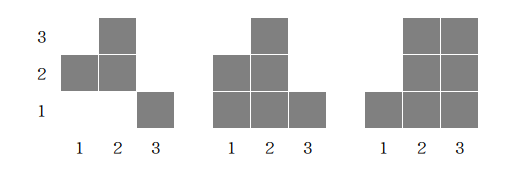
\includegraphics[scale=0.6]{picture/figure1.png}
	\end{figure}
	
	\begin{definition}[轮廓线棋盘]
		对于棋盘 $S$ 和整数 $n$,若 $(\max_{(i,j) \in S} i) \leq n$ 且对于每个 $1 \leq i \leq n$ 均存在非负整数 $a_i$ 使得对于所有正整数 $k$,$(i,k) \in S$ 当且仅当 $k \leq a_i$,则称 $S$ 为\textbf{轮廓线棋盘},记 $S = F(a_1,a_2,\cdots,a_n)$。特别地,允许存在 $a_i=0$,此时第 $i$ 列没有格子。
	\end{definition}
	\begin{definition}[Ferrers 棋盘]
		对于轮廓线棋盘 $S = F(a_1,\cdots,a_n)$,若 $a_1 \leq a_2 \leq \cdots \leq a_n$,则称棋盘 $S$ 为\textbf{Ferrers 棋盘},同时若不存在 $1 \leq i < n$ 满足 $a_i = a_{i+1}$ 则称棋盘 $S$ 为\textbf{严格增 Ferrers 棋盘}。类似地,若 $a_1 \geq a_2 \geq \cdots \geq a_n$,则称棋盘 $S$ 为\textbf{减 Ferrers 棋盘}。
	\end{definition}
	
	在图 \ref{f1} 中,中间和右边的两个棋盘均是轮廓线棋盘,而仅有最右边的棋盘是 Ferrers 棋盘,它们的表示分别是 $F(2,3,1)$ 和 $F(1,3,3)$。
	
	\begin{definition}[$k$-棋盘数\footnote{笔者未在中文文献中找到 "kth rook number" 的翻译。}与棋盘多项式]
		对于棋盘 $S$,定义其子集 $T$ \textbf{合法}当且仅当对于任意两个不同的二元组 $(p_1,q_1),(p_2,q_2) \in T$,$p_1 \neq p_2$ 且 $q_1 \neq q_2$。定义 $R_k(S) = \{T \subseteq S \mid T \text{合法} ,|T| = k\}$,则棋盘 $S$ 的\textbf{k-棋盘数} $r_k(S) = |R_k(S)|$,棋盘 $S$ 的\textbf{棋盘多项式}为 $F_S(x) = \sum_{k=0}^{|S|} r_k(S)x^k$。
	\end{definition}
	\begin{definition}[$k$-命中数\footnote{笔者未在中文文献中找到 "kth hit number" 的翻译。}]
		对于 $n \in \mathbb{N_+}$,定义棋盘 $B_n = \{(i,j) \mid 1 \leq i,j \leq n\}$。对于棋盘 $S \subseteq B_n$ 定义 $H_{k,n}(S) = \{T \in R_n(B_n) \mid |T \cap S| = k \}$,则棋盘 $S$ 的\textbf{k-命中数} $h_{k,n}(S) = |H_{k,n}(S)|$。
	\end{definition}
	
	对应到直观描述上,$k$-棋盘数的组合意义即为在棋盘上放置 $k$ 个车使得任意两个车不在同一行且不在同一列,即互相不攻击的方案数;$k$-命中数的组合意义为所有在 $B_n$ 上放 $n$ 个车使得任意两个车不能互相攻击的方案中放在棋盘 $S$ 上的车有 $k$ 个的方案数。
	
	对于图 \ref{f1} 中左边的棋盘 $S = \{(1,2),(2,2),(2,3),(3,1)\}$,有 $r_0(S) = 1 , r_1(S) = |S| = 4 , r_2(S) = 4 , r_3(S) = 1$,而对于$k \geq 4$,$r_k(S) = 0$;$h_{0,3}(S) = 1 , h_{1,3}(S) = 3,h_{2,3}(S) = 1 , h_{3,3}(S) = 1$。图 \ref{f2} 中描述了 $R_2(S)$ 与 $R_3(S)$ 中的元素,其中放上了车的位置用 X 表示。
	
	\begin{figure}[h]
		\centering
		\caption{$R_2(S)$ 与 $R_3(S)$}
		\label{f2}
		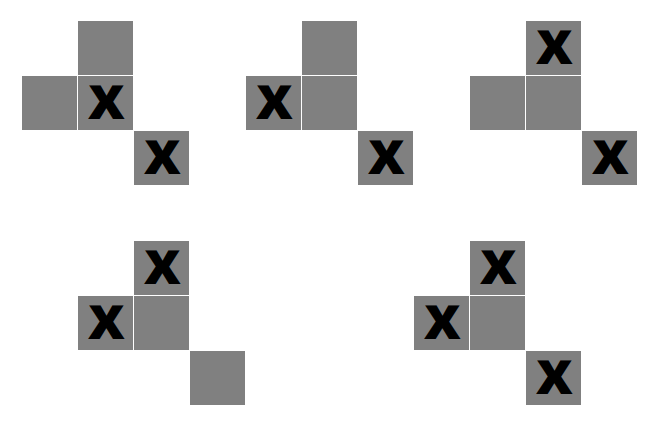
\includegraphics[scale=0.4]{picture/figure2.png}
	\end{figure}
	
	\section{基础定理}
	
	\begin{theorem}[\cite{1998Rook}]\label{fanyan}
		对于棋盘 $S \subseteq B_n$,\begin{equation}
		\sum_{k=0}^n h_{k,n}(S)x^k = \sum_{k=0}^n r_k(S)(n-k)!(x-1)^k
		\end{equation}
	\end{theorem}
	\begin{proof}
	在定理中用 $x+1$ 替换 $x$ 可以得到\begin{equation}
	\sum_{k=0}^n h_{k,n}(S)(x+1)^k = \sum_{k=0}^n r_k(S)(n-k)!x^k
	\end{equation}
	
	对比两侧 $x^i$ 项系数,即需要说明 $\sum_{k=i}^n h_{k,n}(S)\binom{k}{i} = r_i(S)(n-i)!$。
	
	考察 $\sum_{k=i}^n h_{k,n}(S)\binom{k}{i}$ 的组合意义,即为:对于所有命中数 $\geq i$ 的方案,在所有命中的位置中选 $i$ 个作为特殊的命中位置的方案数总和。交换求和顺序,先选择 $i$ 个特殊的命中位置再计算剩余部分的方案数,可以得到相等的结果。选择这 $i$ 个位置的方案数为 $r_i(S)$,而剩余的 $n-i$ 个位置的选择没有其他限制,方案数等于 $n-i$ 行和 $n-i$ 列匹配的方案数,即 $(n-i)!$。
	
	故 $\sum_{k=i}^n h_{k,n}(S)\binom{k}{i} = r_i(S)(n-i)!$,即得 (2) 式 和 (1) 式。
	\end{proof}
	
	定理 \ref{fanyan} 揭示了 $r_k(S)$ 和 $h_{k,n}(S)$ 的联系 ,对于绝大多数的命中数计算问题,需要通过定理 \ref{fanyan} 转化为棋盘数计算问题。
	
	\begin{theorem}[展开定理,\cite{Lu2006}]\label{zhankai}
		给定非空棋盘 $S$,任取 $(p,q) \in S$,设 $S_1 = S - \{(p,q)\} , S_2 = \{(p_1,q_1) \in S \mid p_1 \neq p,q_1 \neq q \}$,有\begin{equation}
			F_S(x) = F_{S_1}(x) + xF_{S_2}(x)
		\end{equation}
	\end{theorem}
	\begin{proof}
		对于确定的 $k$,将 $R_k(S)$ 分为不包含 $(p,q)$ 的方案集合 $R_{k,0}(S)$ 和包含 $(p,q)$ 的方案集合 $R_{k,1}(S)$。$R_{k,0}(S) = R_k(S_1)$,而在 $R_{k-1}(S_2)$ 包含的方案中加入 $(p,q)$ 可得 $R_{k,1}(S)$。
	\end{proof}
	
	直观理解即对于位置 $(p,q)$ 枚举其是否放车,若不放车则这个位置从 $S$ 中删除;否则这个车能够攻击到的所有位置都不能放车,故被删除。如图 \ref{f2-1} 所示,在左侧棋盘 $S$ 中选择 $(3,3)$ 作为位置 $(p,q)$,那么 $S_1$ 和 $S_2$ 分别为中间和右侧的两个棋盘。
	
	\begin{figure}[h]
		\centering
		\caption{展开定理图示}
		\label{f2-1}
		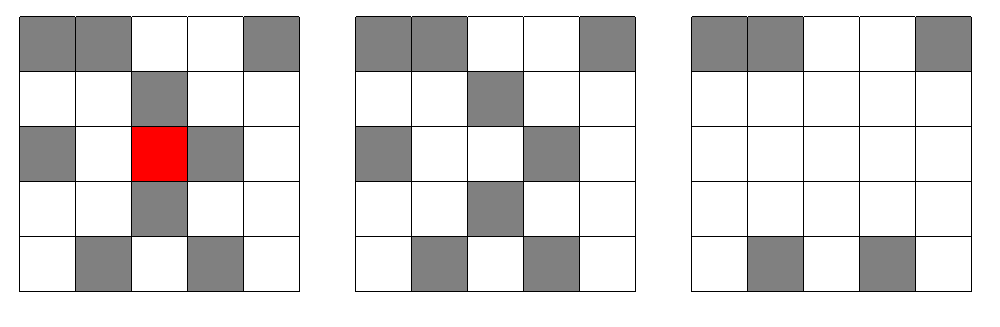
\includegraphics[scale=0.4]{picture/ppt-figure1.png}
	\end{figure}
	
	利用定理 \ref{zhankai} 可以得到易于编程实现的计算棋盘多项式的朴素算法,但效率通常不高。
	
	\begin{theorem}[分离定理,\cite{Lu2006}]\label{fenli}
		对于棋盘 $S$ 和 $S_1 \subseteq S$,设 $S_2 = S - S_1$,若对于任意 $(p_1,q_1) \in S_1 , (p_2,q_2) \in S_2$ 都有 $p_1 \neq p_2,q_1 \neq q_2$,则\begin{equation}
		F_S(x) = F_{S_1}(x)F_{S_2}(x)
		\end{equation}
	\end{theorem}
	\begin{proof}
		对于 $S_1$ 的任一合法子集 $T$ 和 $S_2$ 的任一合法子集 $\overline T$,由于 $S_1$ 和 $S_2$ 的行列不交,因此 $T + \overline T$ 是 $S$ 的合法子集。同时 $S$ 的合法子集 $T+\overline T$ 可恰好分为属于 $S_1$ 的部分 $T$ 和属于 $S_2$ 的部分 $\overline T$。故 $S$ 的合法子集与 $S_1,S_2$ 的合法子集构成的二元组一一对应,则 $r_k(S) = \sum_{i=0}^k r_i(S_1)r_{k-i}(S_2)$,即得式 (4)。
	\end{proof}
	
	图 \ref{f3} 中,编号属于区间 $[1,4]$ 的格子与属于区间 $[5,9]$ 的格子行列无交,因此可以分别算出它们的棋盘多项式最后卷积合并。在部分特殊棋盘中,通过定理 \ref{fenli} 将大棋盘拆成若干个小棋盘有利于简化计算。
	
	\begin{figure}[h]
		\centering
		\caption{分离定理图示}
		\label{f3}
		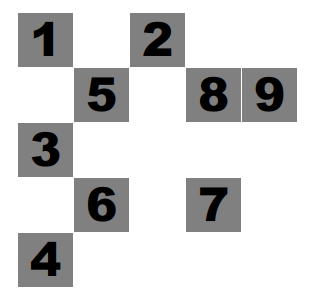
\includegraphics[scale=0.43]{picture/figure3.png}
	\end{figure}
	
	\section{禁区排列问题}
	
	这一部分将介绍两个禁区排列问题。
	
	\begin{problem}[错排问题\footnote{来源:经典问题}]
		给定 $n$,求有多少个 $n$ 阶排列 $\pi$ 满足不存在 $1 \leq i \leq n$ 使得 $i = \pi_i$,答案对大质数取模。$1 \leq n \leq 10^7$。
	\end{problem}
	
	设 $S = \{(1,1),(2,2),\cdots,(n,n)\}$,则错排问题的解为 $h_{0,n}(S)$。由定理 \ref{fanyan} 有 $h_{0,n}(S) = \sum_{i=0}^n r_i(S) (n-i)! (-1)^i$。由于 $S$ 中任意两个格子不在同行或同列,因此 $r_i(S) = \binom{n}{i}$。故有\begin{equation}
	h_{0,n}(S) = \sum_{i=0}^n (-1)^i \binom{n}{i}(n-i)! = n! \sum_{i=0}^n \frac{(-1)^i}{i!}
	\end{equation}
	
	\begin{problem}[夫妻分座问题\footnote{来源:经典问题改编}]
		给定 $n$ 和两个 $n$ 阶排列 $p,q$,对于 $k \in [0,n]$ 求有多少个 $n$ 阶排列 $\pi$ 满足 $\sum_{i=1}^n [\pi_i = p_i \text{或} \pi_i = q_i] = k$,答案对 $998244353$ 取模。$1 \leq n \leq 2\times 10^5$。
	\end{problem}
	
	构造棋盘 $S = \{(i,j) \mid 1 \leq i,j \leq n , j = p_i \text{或}j=q_i\}$,则需要对 $k \in [0,n]$ 计算 $h_{k,n}(S)$。仍使用定理 \ref{fanyan} 转化为计算 $F_S(x)$,但这个棋盘并没有错排问题棋盘的显然的优秀性质。
	
	不妨先考虑一类特殊情况:$n>1,p_i = i,q_i = (i \bmod n) + 1$。此时其直观描述如图 \ref{f4}。
	
	\begin{figure}[h]
		\centering
		\caption{$n=5$ 时特殊情况的图示}
		\label{f4}
		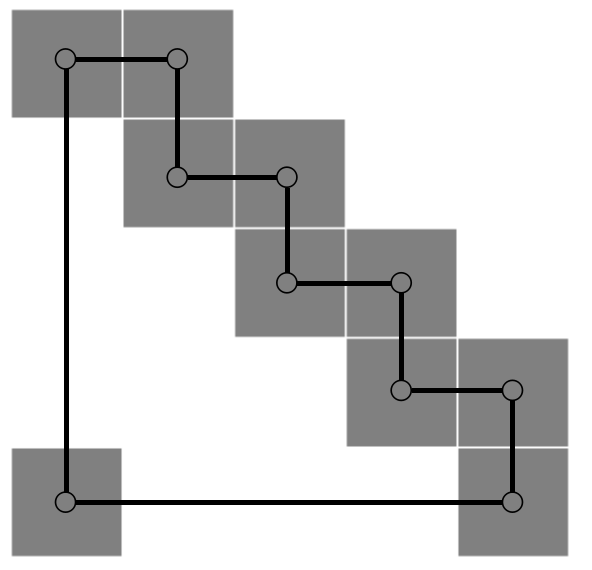
\includegraphics[scale=0.23]{picture/figure4-1.png}
	\end{figure}
	
	对每个格子建一个点,将两个在同行或同列的格子间连一条边,如图 \ref{f4},则其恰好构成长度为 $2n$ 的环,而 $r_k(S)$ 等于在这个环上选 $k$ 个点使得任意两个点不相邻的方案数。
	
	该问题在链上较容易解决,考虑断环成链。对于每个点,强制其不选并计算剩余 $2n-1$ 个点构成的链上选择 $k$ 个点满足任意两个点不相邻的方案数,即计算有多少个递增序列 $1 \leq a_1 < \cdots < a_k \leq 2n-1$ 满足对于所有 $1 \leq i < k,a_{i+1} \neq a_i + 1$。
	
	对于合法序列 $A = \{a_1,\cdots,a_k\}$ 设 $T(A) = \{t_1 = a_1-1,\cdots,t_k = a_k-k\}$,则 $T(A)$ 需要满足严格递增且 $t_0 \geq 0,t_k \leq 2n-k-1$。而满足该条件的序列 $T(A)$ 唯一对应一个合法序列 $A$,故合法的 $A$ 和 $T(A)$ 数量相等。而合法的 $T(A)$ 序列与在 $[0,2n-k-1]$ 中选 $k$ 个数的方案一一对应,故其数量为 $\binom{2n-k}{k}$。
	
	对于 $2n$ 个点均计算一次答案并求和,此时每个选择 $k$ 个点的合法方案都会贡献 $2n-k$ 次,故 $r_k(S) = \frac{2n}{2n-k}\binom{2n-k}{k}$。特殊情况得到解决。
	
	拓展到一般情况,类似图 \ref{f4} 的方式建立一张图,此时每个点的度数为 $0$ 或者 $2$。值得注意的是不会存在度数为 $1$ 的点。图会形成若干个连通块,连通块之间行列无交,根据定理 \ref{fenli} 可以分别计算每个连通块的棋盘多项式然后卷积合并。
	
	度数为 $0$ 的点构成单独的连通块,棋盘多项式为 $x+1$。
	
	其他连通块每个节点度数为 $2$,故其构成一个环,棋盘多项式求解与特殊情况一致。
	
	使用分治 FFT 合并每个连通块的棋盘多项式得到 $r_k(S)$,再使用 FFT 优化二项式反演得到 $h_{k,n}(S)$ 即可解决原问题。复杂度 $O(n \log^2 n)$。 
	
	特别地,笔者对于该问题的另一个特殊情况:$p_i = i , q_i = n-i+1$ 进行了研究,得到了更优复杂度的做法,由于篇幅原因本文不进行阐述,具体内容可见参考文献 \cite{psj}。
	
	\section{Ferrers 棋盘的棋盘多项式}
	
	Ferrers 棋盘由于性质优秀,且与其他的组合工具有密切联系,故一直是棋盘理论中重要的研究对象。本节将会对 Ferrers 棋盘的棋盘多项式进行简单讨论。
	
	\subsection{下降幂棋盘多项式分解定理}
	
	\begin{theorem}[下降幂棋盘多项式分解定理,\cite{1975Rook}]\label{xiajiangmi}
		对于 Ferrers 棋盘 $S = F(a_1,a_2,\cdots,a_n)$,\begin{equation}
		\sum_{k=0}^n r_k(S)x^{\underline{n-k}} = \prod_{k=1}^n (x+a_k-k+1)
		\end{equation}
	\end{theorem}
	\begin{proof}
		式 (6) 两侧均为关于 $x$ 的多项式,故仅需要在无限多个点处证明式 (6) 成立即可证明式 (6) 恒成立。考虑在 $x \in \mathbb{N}$ 处证明。
		
		如图 \ref{f5} 所示,设 $S_x$ 为在棋盘 $S$ 下方加入额外 $x$ 行得到的棋盘。考虑使用两种方法计算 $r_n(S_x)$:
		\begin{figure}[h]
			\centering
			\caption{$S = F(1,3,3)$ 时 $S_x$ 所表示的棋盘}
			\label{f5}
			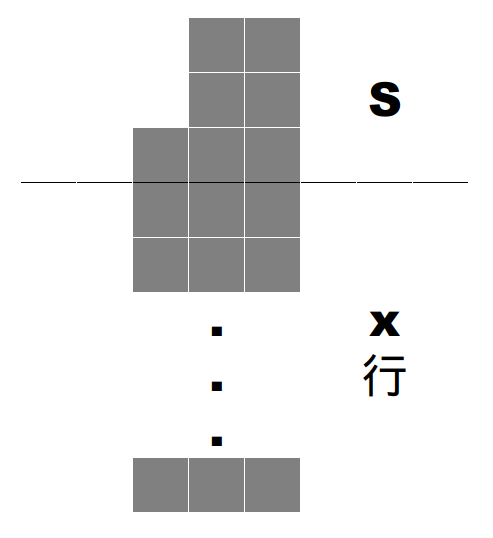
\includegraphics[scale=0.3]{picture/figure5.png}
		\end{figure}
		\begin{enumerate}
			\item 从左往右确定每列的放车位置。
			
			第一列有 $x+a_1$ 个位置可以放车;第二列有 $x+a_2$ 个位置可以放车,但由于第一列放了车且 $a_1 \leq a_2$,因此恰好存在一个位置不能放车,方案数为 $x+a_2-1$;由于前两列的两个车一定不在同一行,故第三列恰有两个位置无法放车,方案数为 $x+a_3-2$……
			
			第 $i$ 列放置时总会由于前 $i-1$ 列放置的车导致 $i-1$ 个位置无法放车,方案数为 $x+a_i-(i-1)$。每一列方案数是独立的,与前面列的具体放置方案无关,故 $$r_n(S_x) = \prod_{k=1}^n (x+a_k-(k-1)) $$
			\item 枚举 $S$ 的合法子集 $T$,计算所有合法方案中与 $S$ 交集为 $T$ 的方案数。
			
			设 $|T| = k$,那么集合 $T$ 中 $k$ 个车对应的列不能再放车,只需要确定剩下 $n-k$ 列的放车位置。而由于 $T$ 恰好是 $S$ 与放车方案的交集,故这 $n-k$ 列的车只能放在额外加入的 $x$ 行内。
			
			类似第一种方法的讨论,在这 $n-k$ 列内依次放车。第一列放车方案数为 $x$,第二列由于第一列的车放车方案数为 $x-1$,第三列放车方案数为 $x-2$……总方案数为 $x^{\underline{n-k}}$。
			
			而选择合法子集 $T$ 的方案数为 $r_k(S)$,故 $$r_n(S_x) = \sum_{k=0}^n r_k(S)x^{\underline{n-k}}$$
		\end{enumerate}
		
		合并两式即得式 (6)。
	\end{proof}
	一般的 Ferrers 棋盘可通过分治 FFT 计算式 (6) 右侧的多项式,然后通过普通多项式转下降幂多项式\footnote{可参考 \href{https://www.luogu.com.cn/problem/P5383}{https://www.luogu.com.cn/problem/P5383}}得到棋盘多项式,复杂度 $O(n \log^2 n)$。
	
	一个更好的做法是在分治 FFT 计算右侧多项式时直接维护下降幂多项式而不是普通多项式,在计算下降幂多项式乘法时使用卷积得到其在 $1,2,\cdots,n$ 处的点值,相乘后卷积还原\footnote{可参考 \href{https://www.luogu.com.cn/problem/P5394}{https://www.luogu.com.cn/problem/P5394}}。复杂度仍为 $O(n \log^2 n)$,但其可以避免普通多项式转下降幂多项式中常数较大的多项式多点求值。
	
	\begin{problem}[Gnutella Chessmaster\footnote{来源:Petrozavodsk Programming Camp Summer 2018 Day 3: MIPT Contest G}]
		给定一个 $n \times n$ 的棋盘,对于 $k \in [1,2n-1]$ 求在棋盘上放 $k$ 个国际象棋中的象使得它们两两互不攻击的方案数,对 $998244353$ 取模。两个象 $(x_1,y_1)$ 和 $(x_2,y_2)$ 互相攻击当且仅当 $|x_1-x_2| = |y_1-y_2|$。$1 \leq n \leq 10^5$。
	\end{problem}
	
	对棋盘进行黑白染色,观察攻击方式可以知道两个位于不同颜色的象不会互相攻击。使用定理 \ref{fenli} 将黑色格子和白色格子的方案数分开计算,最后使用卷积合并。
	
	由于象攻击的方向是斜对角线不易处理,考虑将棋盘旋转 $45^\circ$ ,这样象攻击的方向与车相同,放置的限制也就是两个象不能在同行或同列。图 \ref{f7} 展示了 $n=5$ 的旋转结果,为了更好地描述限制的对应关系,图 \ref{f7} 的黑色棋盘使用了图 \ref{f4} 中描述限制的方法。\begin{figure}[h]
		\centering
		\caption{$n=5$ 时的黑白染色和旋转之后得到的黑白棋盘}
		\label{f7}
		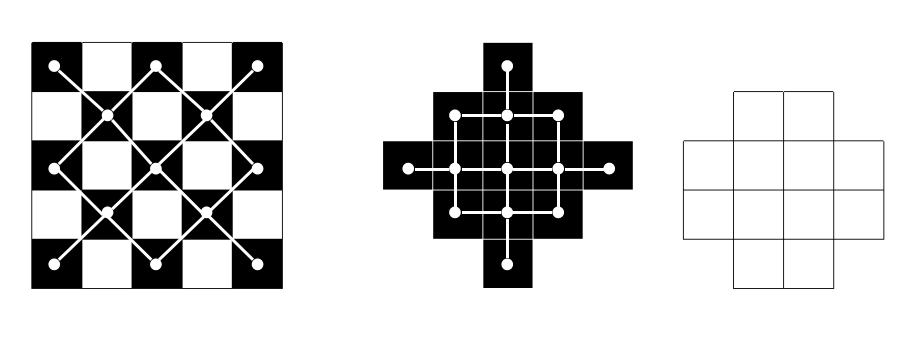
\includegraphics[scale=0.4]{picture/figure7-1.png}
	\end{figure}
	
	由于交换行列不会改变棋盘的棋盘多项式,因此可以先对所有行按照格子个数从大到小排序,再对所有列按照位置个数从小到大排序,可以发现 $n=5$ 时黑色棋盘等于 $F(1,1,3,3,5)$,而白色棋盘等于 $F(2,2,4,4)$。
	
	更一般的性质是:棋盘大小为 $n \times n$ 时两个棋盘都可以通过交换行列变为每一列高度构成的可重集等于对应颜色所有对角线长度构成的可重集的 Ferrers 棋盘,即黑色棋盘为 $F(1,1,3,3,5,5,\cdots)$,白色棋盘为 $F(2,2,4,4,6,6,\cdots)$。由于两个棋盘求解仅有细节上的区别,下文仅考虑黑色棋盘的求解。
	
	对于黑色棋盘,运用定理 \ref{xiajiangmi} 得\begin{equation}
	\begin{split}
	\sum_{k=0}^n r_k(S)x^{\underline{n-k}} &= (x+1)^{\lceil \frac{n}{2} \rceil} x^{\lfloor \frac{n}{2} \rfloor}
	\end{split}
	\end{equation}
	
	朴素实现复杂度 $O(n \log^2 n)$。但注意到右式的单点点值可以 $O(\log n)$ 计算,故可以以 $O(n \log n)$ 的复杂度计算出其在 $0,1,\cdots,n$ 处的点值然后通过卷积得到左侧多项式系数。复杂度优化为 $O(n \log n)$。
	
	\subsection{阶梯棋盘与斯特林数}
	
	\begin{definition}[阶梯棋盘]
		对于 Ferrers 棋盘 $S = F(a_1,a_2,\cdots,a_n)$,若对于所有 $1 \leq i \leq n$ 有 $a_i = i-1$,则称 $S$ 为 $n$ 阶阶梯棋盘,记 $S$ 为 $St_n$。
	\end{definition}

	\begin{figure}[h]
		\centering
		\caption{$St_6$}
		\label{f6}
		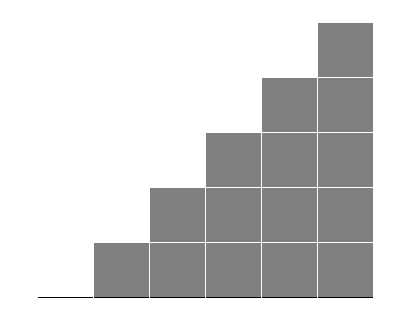
\includegraphics[scale=0.35]{picture/figure6.png}
	\end{figure}

	图 \ref{f6} 描述了 $St_6$。对 $St_n$ 应用定理 \ref{xiajiangmi} 有 \begin{equation}
	\sum_{k=0}^n r_k(St_n) x^{\underline{n-k}} = x^n
	\end{equation}
	
	有 $r_{n-k}(St_n) = {n \brace k}$,即在 $St_n$ 上放 $n-k$ 个车使得任意两个车不能互相攻击的方案数与将 $n$ 个整数划分为 $k$ 个无序集合的方案数一致。考虑在这两个问题之间建立一个双射。
	
	对于集合划分 $S_1,S_2,\cdots,S_k$,将每个集合中的元素从小到大排序。设 $S_i = \{a_1,a_2,\cdots,a_p\}$,其中$a_1<a_2<\cdots<a_p$,则在棋盘的 $(a_2,a_1),(a_3,a_2)\cdots,(a_p,a_{p-1})$ 位置放车。这样得到的放车方案合法且放车数量为 $n-k$。
	
	对于一个 $n-k$ 个车的合法放车方案,若某个车放在 $(p,q)$ 则将 $p,q$ 所在的集合合并,可以得到一个合法的集合划分。由于某个车放在 $(p,q)$ 可推知 $p$ 所在集合中比 $p$ 小的最大元素恰好是 $q$,因此若某个放车方案对应的划分中存在集合 $a_1<a_2<\cdots<a_p$ 则唯一对应的放车方案为 $(a_2,a_1),(a_3,a_2)\cdots,(a_p,a_{p-1})$。这样集合划分和放车方案的两个映射互为逆映射,方案一一对应。
	
	在另一类与棋盘相关的数上 $n$ 阶阶梯棋盘与无符号第一类斯特林数也有关系。
	\begin{definition}
		设 $F_k(S)$ 表示在棋盘 $S$ 上放置 $k$ 个车使得没有两个车在同一列的所有方案构成的集合,$f_k(S) = |F_k(S)|$。
	\end{definition}

	注意相比 $r_k(S)$,$f_k(S)$ 没有两个车不能在同一行的限制。有 
	\begin{theorem}\label{fileplacement}
		对于轮廓线棋盘 $S = F(a_1,a_2,\cdots,a_n)$,
		\begin{equation}
			\sum_{k=0}^n f_{n-k}(S)x^k = \prod_{i=1}^n (x+a_i)
		\end{equation}
	\end{theorem}
	\begin{proof}
		可以这样计算 $f_k(S)$ :选出放车的 $k$ 列,由于没有行限制因此第 $i$ 列方案数是 $a_i$,故 $f_k(S)$ 等于从 $\{a_1,a_2,\cdots,a_n\}$ 中选 $k$ 个数相乘并求和,即 $f_k(S) = [x^{n-k}] \prod_{i=1}^n (x+a_i)$。
	\end{proof}
	
	对 $St_n$ 使用定理 \ref{fileplacement} 有 \begin{equation}
	\sum_{k=0}^n f_{n-k}(St_n)x^k = x^{\overline n}
	\end{equation}
	此时 $f_{n-k}(St_n) = {n \brack k}$,即在 $St_n$ 上放 $n-k$ 个车使得任意两个车不在同一列的方案数等于将 $n$ 个数划分成 $k$ 个圆排列的方案数。考虑在这两个问题之间建立一个双射。
	
	对于某个划分为 $k$ 个圆排列的方案,对每个排列将最小的元素放在开头,然后从 $n$ 至 $1$ 考虑。假设现在在考虑 $i$,若其所在排列中仅有一个元素则删掉这个排列,否则设其在该排列中恰好在它前面的元素为 $v$,则在 $(i,v)$ 放一个车并将 $i$ 从该排列中删掉。这样得到的放车方案恰好放了 $n-k$ 个车,满足每一列至多有一个车且在阶梯棋盘内。
	
	以圆排列 $(162)(35)(4)$ 举例说明操作过程:
	\begin{enumerate}
		\item 对于 $6$,其前驱为 $1$,因此加入车 $(6,1)$ 并删掉 $6$ 得到 $(12)(35)(4)$;
		\item 对于 $5$,其前驱为 $3$,因此加入车 $(5,3)$ 并删掉 $5$ 得到 $(12)(3)(4)$;
		\item 对于 $4$ 和 $3$,它们所在的排列的长度均为 $1$,因此删掉它们,剩余 $(12)$;
		\item $2$ 的前驱是 $1$,故在 $(2,1)$ 上放车。最后 $1$ 自成一个排列将其删掉,过程结束。
	\end{enumerate}
	
	故其对应的放车方案为 $\{(2,1),(5,3),(6,1)\}$。
	
	同时对于一个合法放车方案,按列从小到大考虑,若这一列没有车则新开一个以其为唯一元素的圆排列,否则放在放车的行对应的数字后面,可以得到 $k$ 个圆排列的划分方案,且两个映射互为逆映射。因此圆排列划分与不考虑行限制的放车方案是一一对应的。
	
	对于两类斯特林数,有重要的斯特林反演公式:\begin{equation}
	\sum_{k=x}^y {y \brace k} {k \brack x}(-1)^{k-x} = [x=y]
	\end{equation}
	
	上文给出了 $n \brace k$ 和 $n \brack k$ 在棋盘模型中的组合意义,那么我们可以考虑通过这样的组合意义证明斯特林反演公式。有\begin{equation}
	\begin{split}
	\sum_{k=x}^y {y \brace k} {k \brack x}(-1)^{k-x} &= \sum_{k=x}^y r_{y-k}(St_y) f_{k-x}(St_k)(-1)^{k-x} \\ &= \sum_{k=x}^y \sum_{P \in R_{y-k}(St_y)} \sum_{Q \in F_{k-x}(St_k)}(-1)^{|Q|}
	\end{split}
	\end{equation}
	
	$x=y$ 时容易验证上式等于 1;$x \neq y$ 时,将所有 $(k,P,Q)$ 三元组分成三类:
	\begin{enumerate}
		\item $P$ 的第 $y$ 列放了车;
		\item $P$ 的第 $y$ 列没放车,但 $Q$ 的第 $k$ 列放了;
		\item $P$ 的第 $y$ 列和 $Q$ 的第 $k$ 列都没放车。
	\end{enumerate}
	
	考虑建立 $1$ 类集合和 $2$ 类集合的反号双射,即 $1$ 类集合中的每个三元组与 $2$ 类集合中的某个三元组一一对应,且它们对和式的贡献互为相反数。
	
	具体地,对于某个属于 $1$ 类集合的三元组 $(k,P,Q)$,对棋盘 $P,Q$ 进行如下操作:
	\begin{enumerate}
		\item 将 $P$ 中第 $y$ 列的车删除得到 $P'$,并将 $P'$ 上没有放车的行从下往上从 $1$ 开始编号。记录 $P$ 中第 $y$ 列的车放在新编号下第 $p$ 行。由于 $P'$ 上有 $y-k-1$ 个车,故 $p \in [1,k]$。
		\item 在 $Q$ 中加入 $(k+1,p)$ 得到 $Q'$。
	\end{enumerate}
	则 $(k,P,Q)$ 对应 $(k+1,P',Q')$。由于 $P' \in R_{y-k-1}(St_y),Q' \in F_{k+1-x}(St_{k+1})$,且 $P'$ 的第 $y$ 列没有放车、$Q'$ 第 $k+1$ 列放了车,因此 $(k+1,P',Q')$ 属于 $2$ 类集合。同时 $|Q'| - |Q| = 1$ 且该映射的逆映射容易构造,因此 $1$ 类集合和 $2$ 类集合间存在反号双射。
	
	那么只需要计算 $3$ 类集合的贡献,有 \begin{equation}
	\begin{split}
	\sum_{k=x}^y \sum_{P \in R_{y-k}(St_y)} \sum_{Q \in F_{k-x}(St_k)}(-1)^{|Q|} &= \sum_{k=x}^y \sum_{P \in R_{y-k}(St_{y-1})} \sum_{Q \in F_{k-x}(St_{k-1})}(-1)^{|Q|} \\ &= \sum_{k=x-1}^{y-1} \sum_{P \in R_{(y-1)-k}(St_{y-1})} \sum_{Q \in F_{k-(x-1)}(St_k)}(-1)^{|Q|} \\ &= \sum_{k=x-1}^{y-1} {y-1 \brace k} {k \brack x-1}(-1)^{k-(x-1)}
	\end{split}
	\end{equation}
	
	即将 $x,y$ 减去 $1$ 答案不变。不断减直到 $x=0$,由于 $y>x$ 容易验证该式等于 $0$。
	
	那么通过棋盘的组合意义可以证明斯特林反演公式。
	
	\subsection{棋盘等价类}
	
	\begin{definition}[棋盘等价]
		定义两个棋盘 $S,T$ \textbf{等价}当且仅当对于所有 $i \geq 0$,$r_i(S) = r_i(T)$。
	\end{definition}
	
	对于 Ferrers 棋盘 $S = F(a_1,\cdots,a_n)$,由于在序列 $\{a_1,\cdots,a_n\}$ 的开头加入若干个 $0$ 或删除其开头的若干个 $0$ 不会改变其 $k$-棋盘数,故考虑调整其开头的 $0$ 的数量,即在棋盘前端插入或删除若干空列使得该序列的长度为 $|S| + 1$,得到新的棋盘 $S' = F(a'_1,a'_2,\cdots,a'_{|S|+1})$。此时定义 $B_S = \{b_{S,1} = a'_1,b_{S,2} = a'_2-1,\cdots , b_{S,|S|+1} = a'_{|S|+1}-|S|\}$。注意序列 $B_S$ 的长度总是 $|S| + 1$,而与 $S$ 的列数无关。有
	\begin{theorem}[Ferrers 棋盘的等价判定,\cite{1975Rook}] \label{equal}
		两个 Ferrers 棋盘 $S,T$ 等价当且仅当 $B_S$ 的元素构成的可重集与 $B_T$ 的元素构成的可重集一致。
	\end{theorem}
	\begin{proof}
		由定理 \ref{xiajiangmi},Ferrers 棋盘 $S = F(a_1,\cdots,a_{|S| + 1})$ 的下降幂棋盘多项式为 $\prod_{i=1}^{|S|+1}(x+a_i-i+1)$。注意到 $B_S$ 即 $\{a_i-i+1 \mid 1 \leq i \leq |S|+1\}$ 所构成的可重集,故可以将棋盘 $S$ 的下降幂棋盘多项式改写为 $\prod_i (x+i)^{cnt(B_S , i)}$,其中 $cnt(B_S , i)$ 表示整数 $i$ 在可重集 $B_S$ 中的出现次数。
		
		因此当 $B_S = B_T$ 时,两个棋盘的下降幂棋盘多项式相等,对比系数即得两个棋盘的 $k$-棋盘数相等;同时由于将一个多项式分解为常数乘若干个一次项系数为一的一次式乘积的方式是唯一的,故棋盘 $S,T$ 的下降幂棋盘多项式相等可以推得 $S,T$ 的下降幂棋盘多项式的一次式分解形式相等,即 $B$ 序列对应的可重集相等。
	\end{proof}
	
	由于棋盘等价具有传递性,所以提出对棋盘等价类进行分析的想法是自然的。
	
	首先对 Ferrers 棋盘 $S$ 的序列 $B_S$ 提出引理:
	\begin{lemma}
		对于 Ferrers 棋盘 $S = F(a_1,\cdots,a_{|S|+1})$ 和 $1 \leq i \leq |S| + 1$,$b_{S,i} \leq 0$。
	\end{lemma}
	\begin{proof}
		假设存在 $1 \leq i \leq |S| + 1$ 使得 $b_{S,i} > 0$。此时有 $a_i \geq i$。由 Ferrers 棋盘的定义可得对于所有 $i \leq j \leq |S| + 1,a_j \geq a_i$,故 $|S| =\sum_{k=1}^{|S|+1} a_k \geq \sum_{k=i}^{|S|+1}a_i \geq (|S|+2-i)i$。
		
		而 $(|S|+2-i)i$ 是关于 $i$ 的、二次项系数小于 $0$ 的二次函数,其在区间 $[1,|S|+1]$ 的最小值在区间端点 $1$ 或 $|S| + 1$ 处取到。而将 $i=1$ 和 $i=|S|+1$ 代入得到该式等于 $|S|+1 > |S|$,因此 $|S| \geq (|S|+2-i)i > |S|$,产生矛盾。
		
		故不存在 $b_{S,i} > 0$,引理得证。
	\end{proof}
	由于 Ferrers 棋盘等价判定仅取决于序列 $B$ 元素构成的可重集,故对于 Ferrers 棋盘 $S$,设 $k = -\min_{i=1}^{|S| + 1} b_{S,i}$,考虑将 $B_S$ 中的元素构成的可重集表示为 $0^{c_0}(-1)^{c_1}(-2)^{c_2}\cdots(-k)^{c_k}$ 的形式,表示序列 $B_S$ 中有 $c_i$ 个 $-i$。值得注意的是,由于对于所有 $2 \leq i \leq |S| + 1$,$b_{S,i} - b_{S,i-1} \geq -1$,故对于所有 $0 \leq i \leq k$,$c_i$ 不会等于 $0$。
	\begin{theorem}[\cite{1975Rook}] \label{strictincrease}
		对于非空 Ferrers 棋盘 $S$,恰好存在一个不存在空列的严格增 Ferrers 棋盘与 $S$ 棋盘等价。
	\end{theorem}
	\begin{proof}
		设 $B_S$ 的元素构成的可重集为 $0^{c_0}\cdots(-k)^{c_k}$。可以任意排列该可重集中的元素得到序列 $B'$,只需 $B'$ 满足 $b'_{i+1} - b'_i \geq -1$ 即对应一个 Ferrers 棋盘。而让序列 $B'$ 对应一个严格增 Ferrers 棋盘则需满足对于所有 $i \leq |S|$,$b'_i \neq -i+1$ 等价于 $b'_i \leq b'_{i+1}$。
		
		因此可以将 $B'$ 分成前后两部分,前一部分是从 $0$ 到 $-k$ 的递减序列,后一部分是从 $-k$ 到 $0$ 的不降序列。满足该条件的序列仅有一个,而容易说明将该序列对应的棋盘的前面若干空列删掉之后得到一个严格增 Ferrers 棋盘。
	\end{proof}
	\begin{theorem}[棋盘等价类大小定理,\cite{1975Rook}]\label{equalsize}
		对于可重集 $T = 0^{c_0}\cdots(-k)^{c_k}$,满足 $B_S$ 的元素构成的可重集为可重集 $T$ 的 Ferrers 棋盘 $S$ 的数量为\begin{equation}
		\prod_{i=0}^{k-1} \binom{c_i+c_{i+1}-1}{c_{i+1}}
		\end{equation}
	\end{theorem}
	\begin{proof}
		考虑构造所有可能的序列 $B_S$。先在序列中加入所有 $0$,然后依次加入 $-1,-2,\cdots,-k$。
		
		加入 $-i$ 时,由于序列相邻两项后一项减前一项不能小于 $-1$ 且第一项必须为 $0$,因此 $-i$ 的前驱一定是 $-i$ 或 $-i+1$,即有 $c_{i-1}$ 个位置可将任意多 $-i$ 放在其后面。使用隔板法,放入 $-i$ 的方案数为 $\binom{c_{i-1}+c_i-1}{c_i}$。由于每个数的方案独立,与之前的数在序列中的排列无关,故总方案为每个数的方案的乘积,即为式 (14)。
	\end{proof}
	
	\subsection{分解定理的变体}
	
	这个部分将会定义两个与 $k$-棋盘数类似的量,并研究在 Ferrers 棋盘上新的量对应的棋盘多项式的性质。
	
	\begin{definition}[$m$ 阶 $k$-棋盘数]
		对于棋盘 $S$ 和正整数 $m$,自下而上将每 $m$ 行分成一组,则设棋盘 $S$ 的\textbf{ $m$ 阶 $k$-棋盘数} $r_{m,k}(S)$ 表示在棋盘 $S$ 上放 $k$ 个车使得不存在两个车在同一个行组或同一列的方案数。
	\end{definition}
	
	特别地 $r_{1,k}(S) = r_k(S)$。$m=2$ 时,对于图 \ref{f8} 中的两个放置,左图放置合法而右图放置不合法,因为右图两个车分别在 $1,2$ 行,它们在同一个行组里。而在 $m=1$ 的情况下,两个放置方案均是合法的。
	
	\begin{figure}[h]
		\centering
		\caption{$m=2$ 时,左图棋盘放置是合法的,而右图是不合法的。}
		\label{f8}
		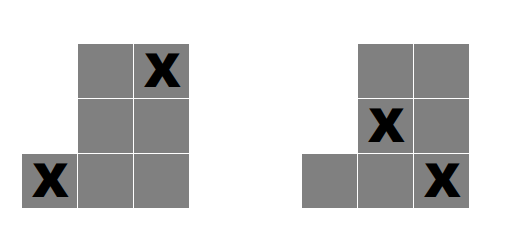
\includegraphics[scale=0.4]{picture/figure8.png}
	\end{figure}
	
	对于 Ferrers 棋盘 $S = F(a_1,a_2,\cdots,a_n)$,将所有非空列按高度分成若干集合 $S_1,S_2,\cdots$,其中 $i \in S_p$ 等价于 $a_i \in [pm+1 , (p+1)m]$,也就是按照每一列能够放置的最高的行组进行分类。设 $\rho_m(S_i) = \sum_{p \in S} a_p - im$。
	
	由于序列 $a$ 单调不降,因此非空的 $S_i$ 会包含一段连续的整数,且随着下标 $i$ 的增加包含的列编号越来越大。
	
	\begin{theorem}[$m$ 阶下降幂棋盘多项式分解定理,\cite{2014m}]\label{mxiajiangmi}
		对于 Ferrers 棋盘 $S = F(a_1,a_2,\cdots,a_n)$ 和正整数 $m$,有\begin{equation}
		\sum_{k=0}^n r_{m,k}(S) x^{\underline{n-k,m}} = \prod_{i=1}^n (x-(i-1)m + v_i)
		\end{equation}
		
		其中若 $a_i = 0$ 则 $v_i = 0$,否则设 $i \in S_p$,若第 $i$ 列是 $S_p$ 的最后一列则 $v_i = pm + \rho_m(S_p)$,否则 $v_i = pm$。
	\end{theorem}
	
	\begin{proof}
		由于式 (15) 两边是关于 $x$ 的多项式,因此只需证明式 (15) 在 $x$ 取无穷多个点处相等即可证明这两个多项式相等。考虑在 $m \mid x$ 的点 $x$ 处证明之。
		
		与图 \ref{f5} 一致地在 $S$ 下面插入额外 $x$ 行得到 $S_x$。$S_x$ 的行组划分仅需在 $S$ 的行组划分的基础上将额外加入的 $x$ 行按顺序分成 $\frac{x}{m}$ 组。用两种方式计算 $r_{m,n}(S_x)$:
		\begin{enumerate}
			\item 枚举 $S$ 的合法子集 $T$ 并计算与 $S$ 的交集为 $T$ 的合法方案数。
			
			设 $|T| = k$,则满足条件的子集 $T$ 的数量为 $r_{m,k}(S)$。剩余 $n-k$ 列的方案可以一列列考虑,类似定理 \ref{xiajiangmi} 的证明,得到其贡献为 $x^{\underline{n-k,m}}$,故 $$r_{m,n}(S_x) = \sum_{k=0}^n r_{m,k}(S)x^{\underline{n-k,m}}$$
			\item 从左到右考虑每个列集合的放车位置。
			
			考虑 $S_p = [s,t]$ 时,先放 $s$ 至 $t-1$ 列的车,且仅考虑这 $t-s$ 列的车放在编号 $\leq pm$ 的行或额外加入的 $x$ 行的情况。对于 $s \leq j < t$,第 $j$ 列共有 $p+\frac{x}{m}$ 组可以放车,其中有 $j-1$ 个组已经放了车,故方案数为 $pm+x-(j-1)m$。
			
			最后考虑第 $t$ 列的放车时,将 $S_p$ 中所有的放车方案分为是否有车放在行组 $[pm+1,(p+1)m]$ 中的两种情况。
			
			对于不放的情况,只需在 $s$ 至 $t-1$ 列的选择上在第 $t$ 列选择不冲突的 $\leq pm$ 的行或额外加入的 $x$ 行,方案数为 $pm+x-(t-1)m$;
			
			对于放的情况,在 $s$ 至 $t-1$ 列的选择上,选择一个位于 $[pm+1,(p+1)m]$ 行组且位于列集合 $S_p$ 的位置放车。若这个放车的位置不在第 $t$ 列,则将其所在列之前放入的车移动至第 $t$ 列,得到有车放在 $[pm+1,(p+1)m]$ 行组的合法方案。
			
			容易证明可以对上述变换构建逆变换,即二元组($s$ 至 $t-1$ 列 的选择方案,$S_p$ 列集合、$[pm+1,(p+1)m]$ 行组的选择方案)与 $S_p$ 中有车放在 $[pm+1,(p+1)m]$ 行组的方案一一对应。此时第 $t$ 列选择的方案数为 $\rho_m(S_p)$。
			
			故第 $t$ 列的方案数为 $x+pm-(t-1)m+\rho_m(S_p)$。
			
			任意两列的方案数互不影响,故 $$r_{m,n}(S_x) = \prod_{i=1}^n (x-(i-1)m+v_i)$$
			\end{enumerate}
			
			合并两式即得式 (15)。
	\end{proof}
	
	\begin{definition}[$\alpha$ 权 $k$-棋盘数]\label{alpha}
		对于棋盘 $S$ 和实数 $\alpha$,定义棋盘 $S$ 的 \textbf{$\alpha$ 权 $k$-棋盘数} $v_{\alpha,k}(S)$ 表示所有在棋盘 $S$ 上放 $k$ 个车使得不存在两个车在同一列的方案的权值和。一个放车方案的权值等于其所有行的权值乘积,一行的权值如下定义:
		\begin{enumerate}
			\item 若该行上放了不超过一个车,则权值为 $1$;
			\item 否则设其放了 $p$ 个车,其权值为 $\alpha (2\alpha-1)(3\alpha-2)\cdots(p\alpha - (p-1))$。
		\end{enumerate}
	\end{definition}
	
	可以注意到的是 $v_{0,k}(S) = r_k(S) , v_{1,k}(S) = f_k(S)$。
	
	\begin{theorem}[$\alpha$ 权下降幂棋盘多项式分解定理,\cite{2000Generalized}]\label{axiajiangmi}
		对于 Ferrers 棋盘 $S = F(a_1,a_2,\cdots,a_n)$ 和实数 $\alpha$,有\begin{equation}
		\sum_{k=0}^n v_{\alpha,k}(S)x^{\underline{n-k,1-\alpha}} = \prod_{i=1}^n (x+a_i-(i-1)(1-\alpha))
		\end{equation}
	\end{theorem}
	\begin{proof}
		将式 (16) 两侧看成关于 $\alpha$ 的 $n$ 次多项式,只需证明对于无穷多个 $\alpha$ 它们相等即可证明式 (16)。考虑在 $\alpha \in \mathbb{N}$ 处证明。
		
		考察新问题:给定棋盘 $S$,从左至右考虑每一列是否放车,若放车则在放车的行上方插入 $\alpha$ 个空行,后面的列决策时可以选择这些新插入的空行,同时在新插入的空行上放车也会插入空行。定义 $v'_{\alpha,i}(S)$ 表示新问题中放 $i$ 个车的方案数,考虑说明 $v'_{\alpha,i}(S) = v_{\alpha,i}(S)$。
		
		建立从新问题方案到原问题方案的映射:对于一个新问题方案,设某个车在第 $i$ 列,放在棋盘 $S$ 的第 $j$ 行或由其直接或间接插入得到的行,则在原问题棋盘中 $(i,j)$ 位置放车。这样一个新问题解对应一个原问题解,而对于一个原问题解,某行有 $p>1$ 个车时,从左往右考虑,第一个车方案数为 $1$、第二个车方案数为 $\alpha$、第三个车方案数为 $2\alpha-1$……总方案数为 $\alpha(2\alpha-1)\cdots(p\alpha-(p-1))$,与该行权值相等。故原问题的方案对应其权值个新问题的方案。因此原问题的方案权值和等于新问题的方案数,即 $v'_{\alpha,i}(S) = v_{\alpha,i}(S)$。
		
		转化为计算新问题之后证明过程与定理 \ref{xiajiangmi} 基本一致,在此不做赘述。
	\end{proof}
	
	\begin{problem}[小 Q 的序列\footnote{来源:LibreOJ 6703,有改动}]
		给定长度为 $n$ 的序列 $a_0,a_1,\cdots,a_{n-1}$ 和一个整数 $\alpha$,定义一个长度为 $k$ 的序列 $p_0,p_1,\cdots,p_{k-1}$ 的权值为 $\prod_{i=0}^{k-1}(p_i+\alpha i)$。对于每个 $0 \leq k \leq n$ 求序列 $\{a_i\}$ 的所有长度为 $k$ 的子序列的权值和,对 $998244353$ 取模。$1 \leq n \leq 10^5$。
	\end{problem}
	
	该问题的经典解法是求解微分方程。接下来我们通过棋盘理论得到一个组合方法。
	
	当序列 $\{a_i\}$ 单调不降的时候,所求解的正是 $F(a_0,\cdots,a_{n-1})$ 的 $(\alpha+1)$ 权棋盘多项式。考虑找到一个单调不降序列 $\{a'_i\}$ 使得两者的答案相等。
	
	在模 $P=998244353$ 意义下任选一个位置 $i$ 进行操作 $a_i \leftarrow a_i + P$ 不会影响答案,因此可以进行若干次该操作直到序列 $\{a_i\}$ 单调不降。此时可以运用定理 \ref{axiajiangmi}。与此同时定理 \ref{axiajiangmi} 右式中进行 $a_i\leftarrow a_i - P$ 不会影响答案,故设长度为 $k$ 的子序列权值和为 $ans_k$,则 $$\sum_{k=0}^n ans_k x^{\underline{n-k,-\alpha}} \equiv \prod_{i=1}^n (x+a_i+(i-1)\alpha)(\bmod\ P)$$
	
	由于该等式并不依赖于 $P$ 的取值,所以在不取模的意义下两者仍然是相等的。
	
	特殊处理 $\alpha = 0$ 的情况,对于其他情况代入 $x=-\alpha y$ 并化简,有
	
	$$\sum_{k=0}^n ans_k(-\alpha)^{n-k} y^{\underline{n-k}} = \prod_{i=1}^n (-\alpha y+a_i+(i-1)\alpha)$$
	
	仍可以使用传统方法计算 $ans_k$ 的取值。复杂度 $O(n \log^2 n)$。
	
	\section{排列降低计数}
	\begin{definition}[降低]
		对于排列 $\pi = \pi_1\pi_2\cdots\pi_n$,定义\begin{gather*}
		Des_{\pi} = \{1 \leq i < n \mid \pi_i > \pi_{i+1}\} , des_{\pi} = |Des_{\pi}| \\
		Des_{\pi,k} = \{1 \leq i < n \mid \pi_i - \pi_{i+1} = k \} , des_{\pi , k} = |Des_{\pi,k}|(k > 0)
		\end{gather*}
		称 $Des_{\pi}$ 为排列 $\pi$ 的\textbf{降低集合},若 $x \in Des_{\pi}$ 则称 $(\pi_x,\pi_{x+1})$ 为一个\textbf{降低对},$des_{\pi}$ 称为 $\pi$ 的\textbf{降低};$Des_{\pi,k}$ 为排列 $\pi$ 的 \textbf {$k$-降低集合},若 $x \in Des_{\pi,k}$ 则称 $(\pi_x,\pi_{x+1})$ 为一个\textbf {$k$-降低对},$des_{\pi,k}$ 称为 $\pi$ 的 \textbf{$k$-降低}。
	\end{definition}
	\begin{definition}[超过数]
		对于排列 $\pi = \pi_1\pi_2\cdots\pi_n$,定义\begin{gather*}
		Exc_{\pi} = \{1 \leq i \leq n \mid \pi_i > i \} , exc_{\pi} = |Exc_{\pi}| \\
		Exc_{\pi,k} = \{1 \leq i \leq n \mid \pi_i - i = k \} , exc_{\pi , k} = |Exc_{\pi,k}|(k > 0)
		\end{gather*}
		称 $Exc_{\pi}$ 为排列 $\pi$ 的\textbf{超过集合},若 $x \in Exc_{\pi}$ 则称 $(\pi_x,x)$ 为一个\textbf{超过对},$exc_{\pi}$ 称为 $\pi$ 的\textbf{超过数};$Exc_{\pi,k}$ 为排列 $\pi$ 的 \textbf{$k$-超过集合},若 $x \in Exc_{\pi,k}$ 则称 $(\pi_x,x)$ 为一个\textbf{$k$-超过对},$exc_{\pi,k}$ 称为 $\pi$ 的 \textbf{$k$-超过数}。
	\end{definition}
	
	我们可以在 $\mathrm{Sym}(n)$ 与 $R_n(B_n)$ 之间建立双射:对于排列 $\pi$ 在所有 $(i,\pi_i) , 1 \leq i \leq n$ 的位置放车。在这样的描述方式下,降低由于涉及相邻两个车的位置关系描述较困难,而超过数仅涉及一个车的行列关系更易描述。下面将要介绍的对排列的变换将在降低和超过数之间建立联系。
	
	\subsection{Foata 第一基本变换}
	\begin{definition}[Foata 第一基本变换]
		对于排列 $\pi$,对其进行 \textbf{Foata 第一基本变换}即依次进行以下操作得到另一个排列 $\pi'$:
		\begin{enumerate}
			\item 将排列写成轮换形式,即写成 $(a_{1,1},\cdots,a_{1,k_1})(a_{2,1},\cdots,a_{2,k_2})\cdots$ 的形式满足 $\pi_{a_{i,j}} = a_{i,(j \bmod k_i) + 1}$。
			\item 将每个轮换中的最大值放到轮换末尾,然后按照轮换中的最大值将轮换从小到大排序;
			\item 将每个轮换看成序列,翻转之后拼接起来得到 $\pi'$。
		\end{enumerate}
	\end{definition}
	
	以 $\pi = 61437258$ 举例说明。其轮换表示为 $(162)(34)(57)(8)$。将每个轮换的最大值放在轮换末尾得到 $(216)(34)(57)(8)$,再按照轮换最大值从小到大排序得到 $(34)(216)(57)(8)$。最后将每个轮换看做序列翻转后拼接得到 $\pi' = 43612758$。
	
	可以通过建立逆变换的方式证明任意两个不同的排列经过该变换不会得到相同的排列:对于排列 $\pi'$,按照前缀最大值将其分段,对于每一段翻转之后看做轮换形式最后还原排列。
	
	如 $\pi' = 43612758$,其中 $4,6,7,8$ 是前缀最大值,故将其划分为 $[43][612][75][8]$,将每个段翻转之后看做轮换形式得到 $(34)(216)(57)(8)$,对应排列 $\pi = 61437258$。
	
	不难证明这两个变换互为逆变换,因此这两个变换在 $\mathrm{Sym}(n)$ 与 $\mathrm{Sym}(n)$ 之间建立了双射。注意到 $\pi$ 中 $(j,i)$ 是一个 $k$-超过对当且仅当 $\pi'$ 中 $(j,i)$ 是一个 $k$-降低对,因此有
	\begin{theorem}\label{des=exc}
		\begin{gather}
		\sum_{\pi \in \mathrm{Sym}(n)} x^{des_\pi} = \sum_{\pi \in  \mathrm{Sym}(n)}x^{exc_{\pi}} \\
		\forall k > 0 , \sum_{\pi \in \mathrm{Sym}(n)} x^{des_{\pi,k}} = \sum_{\pi \in  \mathrm{Sym}(n)}x^{exc_{\pi,k}}
		\end{gather}
	\end{theorem}
	即在一定情况下,降低计数问题和超过数计数问题可以相互转化。由于超过数在棋盘模型中较容易描述,可使用棋盘模型计算超过数的分布,进而得到降低的分布。
	
	\begin{problem}
		给定 $n$ 和 $m$ 个二元组限制,每个二元组限制 $(i,j)$ 均满足 $1 \leq i<j \leq n$,表示在排列中 $i,j$ 相邻且 $i$ 在 $j$ 的前面。对 $k \in [m,n-1]$ 求满足所有二元组限制的 $n$ 阶排列中升高为 $k$ 的排列数量,对 $998244353$ 取模。$n \leq 10^6,n-m \leq 10^5$。定义 $n$ 阶排列 $\pi$ 的升高为 $\sum_{i=1}^{n-1} [\pi_i < \pi_{i+1}]$。\footnote{来源:原创}
	\end{problem}
	
	由于上文中提到的是降低和超过数的关系,所以先将计算对象转化为降低:将 $\pi$ 中的所有数 $x$ 变为 $n-x+1$,然后将所有限制条件 $(i,j)$ 变为 $(n-i+1,n-j+1)$。那么每一个限制 $(p,q)$ 都有 $p>q$,需要计算满足所有二元组限制的排列的降低分布。
	
	考察 Foata 第一基本变换的逆变换过程考虑将问题转化为超过数的计算。由于二元组 $(p,q)$ 有 $p>q$,因此 $q$ 一定不是前缀最大值,在逆变换的分段过程中 $p$ 和 $q$ 一定在一段,即逆变换得到的排列 $\pi$ 一定有 $\pi_q = p$。除此以外没有其他限制条件。
	
	故问题转化为给出若干形如 $\pi_p=q$ 的条件,求满足条件的排列的超过数的分布。对于没有限制的情况,由于排列与棋盘放车有一一对应,考虑构建棋盘模型:如图 \ref{f9} 所示,考虑类似 $St_n$ 的倒三角形式棋盘,其中黑色格子构成棋盘 $S_n$,则容易知道 $h_{k,n}(S_n)$ 为超过数为 $k$ 的排列数。
	
	\begin{figure}[h]
		\centering
		\caption{$n=6$ 时的倒三角棋盘。}
		\label{f9}
		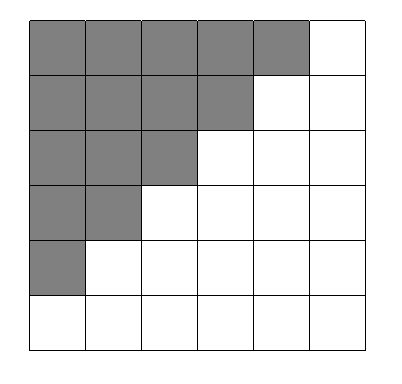
\includegraphics[scale=0.35]{picture/figure9.png}
	\end{figure}
	
	对于有限制的情况,在 $S_n$ 基础上对于每个 $\pi_p = q$ 的条件将第 $p$ 列和第 $q$ 行删除,完成后将没有被删除的行列按顺序进行重标号。则对于结果棋盘上的任一列,在棋盘 $S$ 中的二元组的行编号构成一段右端点为 $n-m$ 的区间,且左端点随着列的增加单调不降。求出每一列的区间长度可以从后往前扫描,复杂度 $O(m)$。
	
	将棋盘旋转不会影响其棋盘多项式,将其旋转 $180^\circ$ 之后得到一个 Ferrers 棋盘。使用定理 \ref{xiajiangmi} 计算其棋盘多项式,再使用定理 \ref{fanyan} 得到 $h_{k,n}(S)$。复杂度 $O(m+(n-m) \log^2 (n-m))$。
	
	~\\
	
	例题中描述了如何使用倒三角棋盘计算满足条件的排列中超过数的分布。我们可以对例题中没有限制的特殊情况进行额外的讨论。
	
	此时需要对每个 $k$ 求 $\sum_{\pi \in \mathrm{Sym}_n} [exc_{\pi} = k]$。由于 $\sum_{\pi \in \mathrm{Sym}_n} [des_{\pi} = k] = {n \bangle k}$,故求的就是欧拉数。与此同时图 \ref{f9} 是求解 $\sum_{\pi \in \mathrm{Sym}_n} [exc_{\pi} = k]$ 的倒三角棋盘 $S_n$,有 ${n \bangle k} = h_{k,n}(S_n)$。将 $S_n$ 旋转 $180^\circ$ 之后得到 $St_n$,而上文讨论了 $r_k(St_n) = {n \brace n-k}$。使用定理 \ref{fanyan},有 $${n \bangle k} = \sum_{i=k}^n (-1)^{i-k} \binom{i}{k} {n \brace n-i} (n-i)!$$
	
	这样我们得到了欧拉数与第二类斯特林数之间的一个经典等式。
	
	\subsection{k-超过数计数}
	
	设 $P_{n,k,p} = \sum_{\pi \in S_n} [exc_{\pi , k} = p]$。$P_{n,k,p}$ 相比超过数的分布计算简单一些,因为其棋盘的形式更简单:设棋盘 $S_{n,k} = \{(1,k+1),(2,k+2),\cdots,(n-k,n)\}$,则 $P_{n,k,p} = h_{p,n}(S_{n,k})$。$S_{n,k}$ 满足不存在两个格子在同行或同列,因此 $r_i(S_{n,k}) = \binom{n-k}{i}$。故
	\begin{theorem}
		\begin{equation}\label{calckexc}
		P_{n,k,p} = \sum_{i=p}^{n-k} (-1)^{i-p} \binom{i}{p} \binom{n-k}{i} (n-i)!
		\end{equation}
	\end{theorem}
	
	$P_{n,k,p}$ 还有一些有趣的性质:
	\begin{theorem}\label{kexc1}
		对于 $0 \leq k < n$,$p \geq 1$,有
		\begin{equation}
		P_{n,k,p} = P_{n-1,k,p-1} + (p+1)P_{n-1,k,p+1}+(n-p-1)P_{n-1,k,p}
		\end{equation}
	\end{theorem}
	\begin{proof}
		考虑在 $\pi \in \mathrm{Sym}(n-1)$ 上按如下方式加入 $n$ 得到 $n$ 阶排列:先将 $n$ 放在 $\pi$ 最后,然后选择一个位置 $i \in [1,n]$,若 $i \neq n$ 则交换 $\pi_i$ 和 $n$得到排列 $\pi'$。考虑该过程的三种结果:
		\begin{enumerate}
			\item $\pi'_{n-k} = n$,即 $exc_{\pi',k} = exc_{\pi,k}+1$。此时 $exc_{\pi,k} = p-1$,且仅有 $i=n-k$ 可以达到该目标,方案数为 $P_{n-1,k,p-1}$。
			\item $\pi'_{n} = i+k$,即 $exc_{\pi',k} = exc_{\pi,k}-1$。此时 $exc_{\pi,k} = p+1$,且这 $p+1$ 个位置作为 $i$ 都合法,方案数为 $(p+1)P_{n-1,k,p+1}$;
			\item 两种情况都没有发生,即 $exc_{\pi',k} = exc_{\pi,k}$。此时 $exc_{\pi,k} = p$,且 $n-1-p$ 个没有贡献 且不是 $n-k$ 的的位置作为 $i$ 均合法,方案数为 $(n-p-1)P_{n-1,k,p}$。
		\end{enumerate}
		合并三者即可得到式 (20)。
	\end{proof}
	作为定理 \ref{kexc1} 在 $p=0$ 处的补充,有
	\begin{theorem}\label{kexc2}
		对于 $0 \leq k < n$,\begin{equation}
		P_{n,k,0} = (n-1)P_{n-1,k,0}+(n-k-1)P_{n-2,k,0}
		\end{equation}
	\end{theorem}
	\begin{proof}
		沿用定理 \ref{kexc1} 的增量计算方式。考虑两种 $exc_{\pi,k}$ 的可能:
		\begin{enumerate}
			\item $exc_{\pi,k} = 0$,此时只需要 $i \neq n-k$ 就合法,贡献为 $(n-1)P_{n-1,k,0}$;
			\item $exc_{\pi,k} = 1$,此时仅有一个 $i$ 合法。对于这样的排列 $\pi$,在棋盘 $S_{n-1,k}$ 上将命中的格子所在行列删掉然后重标号行列,该方案对 $P_{n-2,k,0}$ 产生贡献。同时对于 $P_{n-2,k,0}$ 的每个方案,都有 $n-1-k$ 种方式加入被删掉的位置使得 $exc_{\pi,k} = 1$。故方案数为 $(n-k-1)P_{n-2,k,0}$。
		\end{enumerate}
	将两者合并即可得到式 (21)。
	\end{proof}
	\begin{theorem}\label{kexc3}
	对于 $0 \leq k < n$,有\begin{equation}
	P_{n,k,0} = k!\sum_{r=0}^k \binom{k}{r} \binom{n-k}{k-r} P_{n-k,k-r,0}
	\end{equation}
	\end{theorem}
	\begin{proof}
		使用棋盘理论解决。由于 $S_{n,k}$ 仅在前 $n-k$ 列存在元素,因此考虑枚举最后 $k$ 列的情况。
		
		枚举最后 $k$ 列有 $r$ 个车放在 $1 \sim k$ 行,删掉它们所在的行列时不会删掉 $S_{n,k}$ 中的格子,而剩余 $k-r$ 个车删除行列时会删掉一个格子。选择不删的 $r$ 行的方案数为 $\binom{k}{r}$;选择删的 $k-r$ 行的方案数为 $\binom{n-k}{k-r}$;给最后 $k$ 列分配行的方案数为 $k!$。
		
		删掉这 $k$ 行 $k$ 列后重编号行列,此时还有 $n-k$ 列没有确定,新的限制棋盘 $S'$ 满足 $|S'| = n-r$,由于 $S'$ 仍满足任意两个格子不在同行或同列,可以通过交换行列使得 $S' = S_{n-k,k-r}$,故剩余的方案数为 $P_{n-k,k-r,0}$。
		
		对于所有 $r$ 将每一步的方案数相乘并求和,可以得到式 (22)。
	\end{proof}
	\begin{theorem}\label{kexc4}
		对于 $s \leq k< n$,有
		\begin{equation}
		P_{n,k,s} = \binom{n-k}{s} P_{n-s,k,0}
		\end{equation}
	\end{theorem}
	\begin{proof}
		这个的证明相对简单:恰好有 $s$ 个命中棋盘 $S_{n,k}$,枚举这 $s$ 个位置,有 $\binom{n-k}{s}$ 种情况;对于每种情况将 $s$ 个车所在的行列删掉,剩下 $n-k$ 列要选择,有 $n-s-k$ 个限制的位置,因此删掉行列之后的方案数就是 $P_{n-s,k,0}$。
	\end{proof}
	\subsection{X-Y 降低计数}
	\begin{definition}
		给定数集 $X,Y$,对于 $n$ 阶排列 $\pi$,设 \begin{gather*}
		Des_{\pi,X,Y} = \{1 \leq i < n \mid \pi_i > \pi_{i+1},\pi_i \in X , \pi_{i+1} \in Y\},des_{\pi,X,Y}=|Des_{\pi,X,Y}| \\
		Exc_{\pi,X,Y} = \{1 \leq i < n \mid \pi_i > i,\pi_i \in X , i \in Y\},exc_{\pi,X,Y} = |Exc_{\pi,X,Y}|
		\end{gather*}
		称 $Des_{\pi,X,Y}$ 为排列 $\pi$ 的 \textbf{$X-Y$ 降低集合},若 $x \in Des_{\pi,X,Y}$ 则称 $(\pi_x,\pi_{x+1})$ 为一个 \textbf{$X-Y$ 降低对},$des_{\pi,X,Y}$ 称为 $\pi$ 的 \textbf{$X-Y$ 降低};称 $Exc_{\pi,X,Y}$ 为排列 $\pi$ 的 \textbf{$X-Y$ 超过集合},若 $x \in Exc_{\pi,X,Y}$ 则称 $(\pi_x,x)$ 为一个 \textbf{$X-Y$ 超过对},$exc_{\pi,X,Y}$ 称为 $\pi$ 的\textbf{ $X-Y$ 超过数}。
	\end{definition}
	
	例如 $X=\{2,3,5\},Y=\{1,3,4\}$ 时,排列 $53142$ 的 $X-Y$ 降低对有 $(5,3)$ 和 $(3,1)$。注意 $(4,2)$ 虽然是降低对,但 $4 \not\in X$ 所以其不是 $X-Y$ 降低对。
	
	通过 Foata 第一基本变换同样可以得到 $des_{\pi,X,Y}$ 和 $exc_{\pi,X,Y}$ 的双射关系:
	
	\begin{theorem}\label{desxy=excxy}
		对于 $X,Y \subseteq [1,n] \cap \mathbb{Z}$,有\begin{equation}
		\sum_{\pi \in \mathrm{Sym}_n} x^{des_{\pi,X,Y}} = \sum_{\pi \in \mathrm{Sym}_n} x^{exc_{\pi,X,Y}}
		\end{equation}
	\end{theorem}
	
	计算 $exc_{\pi,X,Y}$ 仍然可以使用棋盘模型:设 $S_{X,Y} = \{(i,j) \mid i \in Y , j \in X , i < j \}$,则 $\sum_{\pi \in \mathrm{Sym}_n} [exc_{\pi,X,Y} = p] = h_{p,n}(S_{X,Y})$。图 \ref{f10} 的左侧棋盘展示了 $X=\{2,3,5,7,8\},Y=\{1,2,4,5,6\}$ 时的棋盘 $S_{X,Y}$。
	
	\begin{figure}[h]
		\centering
		\caption{$X=\{2,3,5,7,8\},Y=\{1,2,4,5,6\}$ 时的棋盘 $S_{X,Y}$ 和交换行列后得到的 Ferrers 棋盘 $F(0,0,0,2,2,3,4,5)$。}
		\label{f10}
		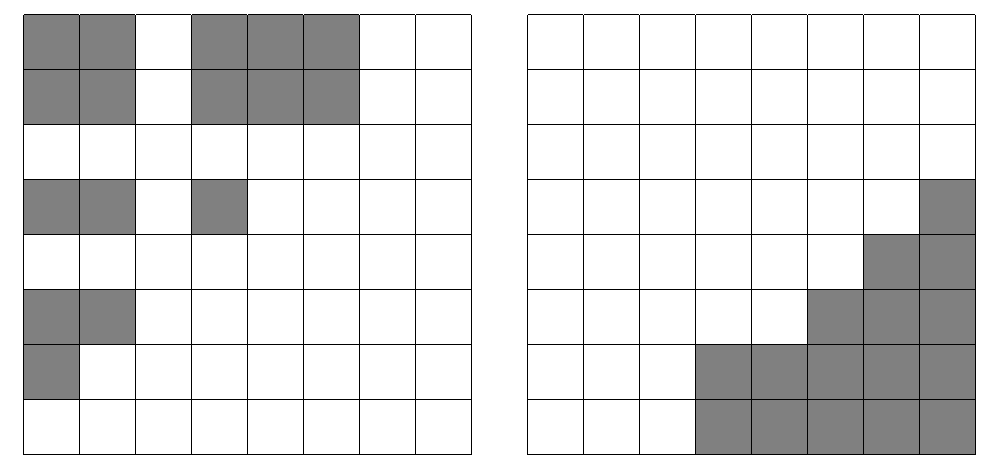
\includegraphics[scale=0.3]{picture/figure10.png}
	\end{figure}
	
	对于这样的棋盘,一个特殊的性质是按照格子个数从小到大排序,可以得到一个 Ferrers 棋盘,如图 \ref{f10} 的右侧棋盘所示。因此我们仍然可以使用定理 \ref{xiajiangmi} 和定理 \ref{fanyan} 来计算对于给定的 $s$,$\sum_{\pi \in \mathrm{Sym}_n} [des_{\pi,X,Y} = s]$ 的值。
	
	由定理 \ref{strictincrease},每个 Ferrers 棋盘恰有一个无视空列情况下的严格增 Ferrers 棋盘与其对应,而当该严格增棋盘的列高为 $a_1<a_2<\cdots<a_p$ 时,可以通过翻转并交换行列得到该棋盘等价于 $S_{\{a_1+1,a_2+1,\cdots,a_p+1\} , \mathbb{N}}$。故有
	\begin{theorem}\label{X'}
		对于任意数集 $X,Y$ 均存在恰好一个数集 $X'$ 使得 \begin{equation}
		\sum_{\pi \in \mathrm{Sym}_n} x^{des_{\pi,X,Y}} = \sum_{\pi \in \mathrm{Sym}_n} x^{des_{\pi,X',\mathbb{N}}}
		\end{equation}
	\end{theorem}
	
	对于图 \ref{f10} 中的例子,通过定理 \ref{strictincrease} 的构造证明,可以得到与 $F(2,3,4,5,5)$ 等价的棋盘是 $F(1,2,3,4,6)$。图 \ref{f11} 中给出了图 \ref{f10} 对应棋盘的等价严格增 Ferrers 棋盘和其翻转、交换行列之后得到的棋盘 $S_{\{2,3,4,5,7\},\mathbb{N}}$。
	
	\begin{figure}[h]
		\centering
		\caption{等价的严格增 Ferrers 棋盘和 $S_{\{2,3,4,5,7\},\mathbb{N}}$}
		\label{f11}
		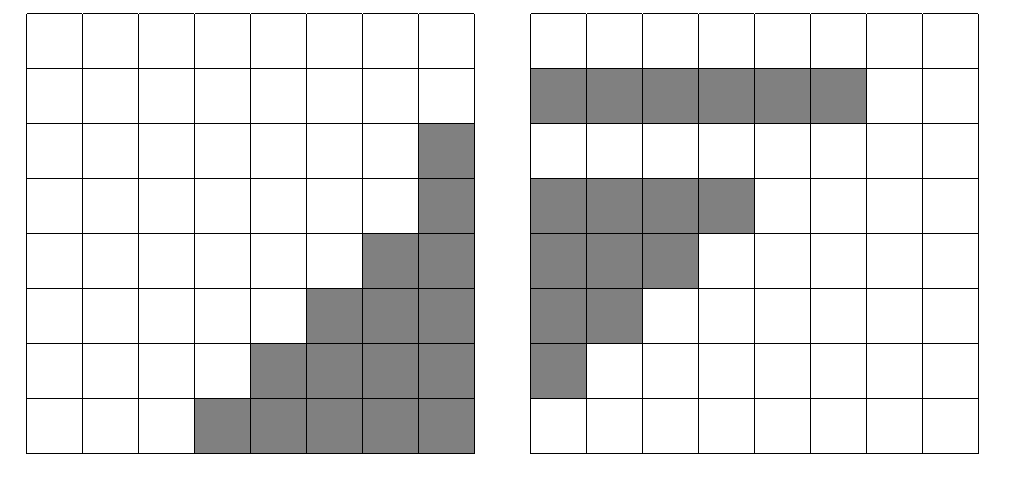
\includegraphics[scale=0.3]{picture/figure11.png}
	\end{figure}
	
	最后,在参考文献 \cite{2008Counting} 中给出了计算 $\sum_{\pi \in \mathrm{Sym}_n} [des_{\pi,X,Y} = s]$ 的公式,但由于其证明没有使用棋盘理论,故仅在此提出不做过多说明。感兴趣的读者可自行阅读参考文献 \cite{2008Counting}。
	\section{Ferrers 棋盘的排列逆序对计数}
	
	在 Atcoder Grand Contest 中已经出现了轮廓线棋盘排列逆序对个数和的问题\footnote{Atcoder Grand Contest 023 E. Inversion}。其给出的标准算法不基于棋盘理论,故在本文中不进行阐述,但由于该算法需要使用到交换求和顺序的方式,故拓展性不强。下面介绍的 q-analogue 理论虽然只能在 Ferrers 棋盘上进行计算,但其基于对每个排列进行逆序对数的带权,具有更强的拓展性。
	\subsection{k-棋盘数的 q-analogue 形式}
	
	q-analogue 理论是一类公式的拓展方式。它需要我们引进一些新的符号。
	
	对于 $n \in \mathbb{R}$,定义 \begin{equation*}
	[n]_q = \frac{1-q^n}{1-q}
	\end{equation*}
	
	其中 $q$ 为形式元。特别地,在 $n \in \mathbb{N}$ 时,可以发现 $[n]_q = 1+q+\cdots+q^{n-1}$。
	
	在后面的 q-analogue 等式中,可以将 $q$ 代入任一使得和式收敛的常数。特别地,约定代入 $q=1$ 时,对于任意 $n \in \mathbb{R}$,$[n]_1 = n$。同时定义 q-analogue 下降幂 $$[n]_q^{\underline k} = [n]_q[n-1]_q\cdots[n-k+1]_q$$
	
	\begin{definition}[棋盘放车方案的权值\footnote{大部分英文文献将其定义为逆序对数 $inv$,但其与对应排列的逆序对数并不相同,为了不产生混淆这里使用权值代替。}]
		对于 Ferrers 棋盘 $S = F(a_1,a_2,\cdots,a_n) \subseteq B_n$ 和任一合法放车方案 $T \subseteq S$,对于 $T$ 中的每一个车 $(i,j)$,在棋盘 $S$ 中对所有满足 $i < k \leq n$ 的位置 $(k,j)$ 和满足 $1 \leq k < j$ 的位置 $(i,k)$ 打上标记。设 $C_S(T)$ 为做完上述操作后 $S$ 中没有被打标记且没有放车的格子数量,则定义 $T$ 在棋盘 $S$ 中的\textbf{权值} $val_S(T) = |C_S(T)|$。
	\end{definition}
	
	需要注意的是这里定义的权值与定义 \ref{alpha} 中定义的权值不同。
	
	如图 \ref{f12} 所示,左侧棋盘为棋盘 $S = F(1,2,2,4,4)$ 的一个放车的方案 $T=\{(2,1),(3,2),(5,4)\}$,而右图展示了对其进行标记操作之后对应的棋盘,其中 M 表示被标记,O 表示既不被标记也没有放车。图上共有 $4$ 个 O 因此 $val_S(T) = 4$。
	
	\begin{figure}[h]
		\centering
		\caption{一个放车方案和其对应的标记和权值}
		\label{f12}
		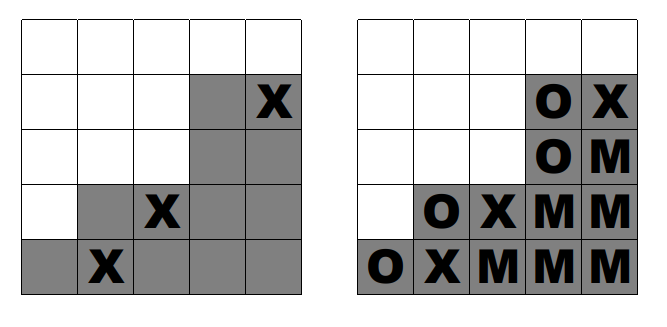
\includegraphics[scale=0.4]{picture/figure12.png}
	\end{figure}
	
	\begin{definition}[正序对,逆序对]
		对于排列 $\pi \in \mathrm{Sym}_n$,定义$$
		coinv_{\pi} = |\{(i,j) \mid i < j , \pi_i < \pi_j \}|,inv_{\pi} = |\{(i,j) \mid i<j,\pi_i>\pi_j \}|
		$$
		分别表示排列 $\pi$ 的正序对数和逆序对数。
	\end{definition}

	对于排列 $\pi$ 和其对应的棋盘放置方案 $T$,若 $T \subseteq S$,可以找到 $val_S(T)$ 与 $coinv(\pi)$ 之间的关系:
	\begin{theorem}\label{val=coinv}
		对于 $n$ 阶排列 $\pi$ 和 Ferrers 棋盘 $S = F(a_1,a_2,\cdots,a_n) \subseteq B_n$,若 $T = \{(i,\pi_i) \mid 1 \leq i \leq n\} \subseteq S$,则\begin{equation}
		val_S(T) + \sum_{i=1}^n n-a_i = coinv(\pi)
		\end{equation}
	\end{theorem}
	\begin{proof}
		由于棋盘 $S$ 是 Ferrers 棋盘,所以棋盘 $S$ 外的格子一定不会被标记,所以 $val_S(T) + \sum_{i=1}^n n-a_i$ 表示的就是 $B_n$ 中没有被标记的格子数量。
		
		对于 $B_n$ 中一个没有被标记且没有放车的格子 $(i,j)$,由于 $|T| = n$,故此时有 $\pi_i < j$,$\pi^{-1}_j > i$,其中 $\pi^{-1}_j$ 表示 $j$ 在排列 $\pi$ 中的位置。那么 $(i,\pi^{-1}_j)$ 此时形成了一个正序对。与此同时一个正序对 $(i,j)$ 也会对应一个没有被标记且没有放车的格子 $(i,\pi_j)$,因此正序对集合与没有被标记的格子的集合一一对应,故有式 (26)。
	\end{proof}

	同时由于有 $coinv(\pi) + inv(\pi) = \binom{n}{2}$,因此 $inv(\pi)$ 与 $val_S(T)$ 的关系是简单的。故通过对 $k$-棋盘数的计算带权来做排列逆序对计数问题是很有发挥空间的。
	
	\begin{definition}[k-棋盘数的 q-analogue 形式]
		对于 Ferrers 棋盘 $S = F(a_1,a_2,\cdots,a_n) \subseteq B_n$,定义 \textbf{$S$ 的 q-analogue $k$-棋盘数} \begin{equation}
			[r_k(S)]_q = \sum_{T \in R_k(S)} q^{val_S(T)}
		\end{equation}
	\end{definition}
	
	当 $q=1$ 时,其定义与 $k$-棋盘数 $r_{k}(S)$ 一致。这也是 q-analogue 理论在进行拓展的时候始终满足的一个特性:当 $q=1$ 时可以得到未进行拓展时就已经得出的定义和结论。
	
	\subsection{q-analogue 形式下的分解定理}
	
	对定理 \ref{xiajiangmi} 在 q-analogue 形式下进行拓展。
	
	\begin{theorem}[q-analogue 下降幂棋盘多项式分解定理,\cite{2004Rook}]\label{q-xiajiangmi}
		对于 Ferrers 棋盘 $S = F(a_1,a_2,\cdots,a_n) \subseteq B_n$,有\begin{equation}
		\sum_{k=0}^n [r_k(S)]_q [x]_q^{\underline{n-k}} = \prod_{i=1}^n [x+a_i-i+1]_q
		\end{equation}
	\end{theorem}
	\begin{proof}
		将式 (28) 左右看做关于 $x$ 的 $n$ 次多项式,因此只需要在无限多个点 $x$ 上证明式 (28) 成立即可证明式 (28) 恒成立。考虑在 $x \in \mathbb{N}$ 上证明。
		
		如图 \ref{f5} 在棋盘 $S$ 下面加上 $x$ 行得到棋盘 $S_x$。使用两种方式计算 $[r_n(S_x)]_q$:
		\begin{enumerate}
			\item 枚举 $S$ 的合法子集 $T$,计算所有合法方案中与 $S$ 交集为 $T$ 的方案的权值和。
			
			设 $|T| = k$,由于额外加入的 $x$ 行不会影响到棋盘 $S$ 中的标记,故 $S$ 上没有被标记且没有放车的格子数量是 $val_S(T)$。
			
			剩余 $n-k$ 列从左往右依次考虑。第一列有 $x$ 个位置可以放车,而决定了放车位置后在这 $x$ 个位置中恰好在其上方的所有格子可以直接贡献到权值。因此从上往下在这些格子上放车权值会增加 $0,1,2,\cdots,x-1$,因此第一列贡献是 $1+q+\cdots+q^{x-1} = [x]_q$。第二列有 $x-1$ 个位置可以放车,其中从上往下考虑在这些格子上放车权值会增加 $0,1,2,\cdots,x-2$,因此第二列的贡献是 $[x-1]_q$。
			
			类似考虑,第 $i$ 列的贡献为 $[x-i+1]_q$。故子集 $T$ 的贡献为 $q^{val_S(T)} [x]_q^{\underline{n-k}}$。对于 $|T| = k$ 的所有 $T$ 求和,它们的 $q^{val_S(T)}$ 的和为 $[r_k(S)]_q$,故一个 $k$ 的贡献为 $[r_k(S)]_q[x]_q^{\underline{n-k}}$。对所有 $0 \leq k \leq n$ 求和,有 $$[r_n(S_x)]_q = \sum_{k=0}^n [r_k(S)]_q(S) [x]_q^{\underline{n-k}}$$
			\item 从左往右考虑每一列放车对权值的影响。
			
			考虑到第 $i$ 列时,其有 $x+a_i-i+1$ 个位置可以放车。与前面类似地,当其确定了放在哪个位置之后,在这 $x+a_i-i+1$ 个格子中在其上方的所有格子可以直接贡献到权值。故第 $i$ 列的贡献为 $q^0+\cdots+q^{x+a_i-i} = [x+a_i-i+1]_q$,总贡献为每一列的贡献和的乘积,即 $$[r_n(S_x)]_q = \prod_{i=1}^n [x+a_i-i+1]_q$$
		\end{enumerate}
	
		合并两式即得式 (28)。
	\end{proof}
	
	定理 \ref{q-xiajiangmi} 在代入 $q=1$ 时即为定理 \ref{xiajiangmi}。特别地,可以代入 $x=0$,由于 $[0]_q = 0$,有
	\begin{lemma}[\cite{1986Q}]
		对于 Ferrers 棋盘 $S = F(a_1,a_2,\cdots,a_n) \subseteq B_n$,有\begin{equation}
		[r_n(S)]_q = \prod_{i=1}^n [a_i-i+1]_q
		\end{equation}
	\end{lemma}
	这样就得到了 $\sum_{T \in R_n(B_n),T \subseteq S} q^{val_S(T)}$ 的封闭形式,即可以得到所有满足对应棋盘放车方案落在 $S$ 内的排列 $\pi$ 的逆序对数分布。
	
	由于该式对于任意常数 $q$ 是收敛的,因此也可以在该式中代入 $q$ 计算所有满足对应棋盘放置方案在 $S$ 内的排列 $\pi$ 的逆序对带权和。计算所有满足条件的排列的逆序对个数和则可以将式 (29) 两侧看成关于 $q$ 的多项式,对 $q$ 求导之后再代入 $q=1$。
	
	同时注意到 $coinv(\pi) = inv(\pi^r)$,其中 $\pi^r$ 表示将 $\pi$ 翻转得到的排列,故对于减 Ferrers 棋盘也有类似的公式。
	
	\section{Ferrers 棋盘的排列环数计数}
	
	\subsection{问题引入}
	
	\begin{problem}[数圈圈\footnote{来源:2021 集训队互测 Round 1 C,\href{https://uoj.ac/problem/597}{https://uoj.ac/problem/597}}]
	给定整数 $n,y$ 和一个长度为 $n$ 的整数序列 $A = \{a_1,a_2,\cdots,a_n\}$,保证序列 $A$ 单调不减或单调不增。
	
	构建有向图 $G(V,E)$,其中 $V = \{1,2,\cdots,n\}$,$E = \{(i,j) \mid 1 \leq i,j \leq n, a_i \geq j\}$。注意图 $G$ 中可能包含自环。
	
	定义边子集 $T \subseteq E$ 合法当且仅当图 $G'(V,T)$ 中每个点的入度和出度不超过 $1$,自环对对应点的入度和出度均贡献 $1$。定义一个合法边子集 $T$ 的权值为 $y^{\mathrm{cycle}(T)}$,其中 $\mathrm{cycle}(T)$ 表示图 $G'(V,T)$ 的环数,自环是一个环。
		
	特别地,本题认为 $0^0=1$。
	
	对于所有整数 $0 \leq k \leq n$,求所有大小为 $k$ 的合法边子集的权值和,对 $998244353$ 取模。$1 \leq n \leq 10^5,0 \leq a_i \leq n , 0 \leq y < 998244353$。
	\end{problem}

	本题为笔者为 2021 年集训队互测命制的题目,由于互测的整体题目难度较高,本题得分率较低,其中定理 \ref{xiajiangmi} 的部分分也鲜有选手得到。下文将讨论的定理  \ref{increasecoverfac}、定理 \ref{uprightcoverfac} 和定理 \ref{decrease=upright} 是解决该问题将会用到的定理。
	
	\subsection{有向图的覆盖多项式}
	
	直接使用棋盘多项式的相关算法计算排列环数相关问题不太现实,因为棋盘数和棋盘多项式并没有记录与环有关的信息。因此需要对棋盘多项式的定义进行拓展。
	
	注意到可以对 $B_n$ 的所有子集和 $n$ 个点的允许有自环但不能有重边的有向图建立双射:对于 $S \subseteq B_n$,若 $(i,j) \in S$ 则在有向图中从 $i$ 到 $j$ 连一条边。因此可以借助有向图上的工具来解决棋盘问题。
	
	\begin{definition}[有向图的覆盖多项式,\cite{1995On}]
		对于 $n$ 个点的有向图 $G$,定义其\textbf{覆盖多项式}\begin{equation}
		C(G,x,y) = \sum_{p \geq 0} \sum_{q \geq 0} c_G(p,q) x^{\underline p}y^q
		\end{equation}
		
		其中 $c_G(p,q)$ 表示用恰好 $p$ 条链和恰好 $q$ 个环覆盖所有点恰好一次的方案数。一个点可以构成一条链,一个自环可以构成一个环。两个覆盖方案不同当且仅当使用的边集不同。
	\end{definition}
	
	举例说明:对于 $n=2$,$G$ 中包含边 $(1,2),(2,1)$ 的有向图 $G$,有四种覆盖方案:
	\begin{enumerate}
		\item $\{1\},\{2\}$ 两条链;
		\item $\{1,2\}$ 一条链;
		\item $\{2,1\}$ 一条链;
		\item $\{1,2,1\}$ 一个环。
	\end{enumerate}

	因此 $C(G,x,y) = x^{\underline 2}+x^{\underline 1}+x^{\underline 1}+y^1 = x^2+x+y$。
	
	有向图的覆盖多项式与对应棋盘的棋盘多项式之间有重要的联系:
	\begin{theorem}[\cite{1995On}]\label{cover=xiajiangmi}
		对于棋盘 $S \subseteq B_n$,设有向图 $G$ 为棋盘 $S$ 对应的有向图,则
		\begin{equation}
		C(G,x,1) = \sum_{k=0}^n r_k(S)x^{\underline{n-k}}
		\end{equation}
	\end{theorem}
	\begin{proof}
		对比其 $x^{\underline {n-k}}$ 次项系数,即需要证明 \begin{equation}
		r_k(S) = \sum_{q \geq 0} c(G,n-k,q)
		\end{equation}
		
		对于某个有 $n-k$ 条链的覆盖方案,恰好有 $n-k$ 个点没有出边。且每个点的入出度均不超过 $1$,故其对应的棋盘每行列仅有一个格子,总共占据 $k$ 个格子,故其对应一个 $k$ 个车的合法放置方案。与此同时对于一个 $k$ 个车的合法放置方案可以通过上文构建的双射得到一个 $n-k$ 个点没有出度的图,即恰好用 $n-k$ 条链覆盖的方案。
		
		因此用 $n-k$ 条链、环数不限的方式覆盖图 $G$ 的方案数等于在 $S$ 上放 $k$ 个车的合法方案数,此时有式 (32) 成立,故式 (31) 成立。
	\end{proof}
	
	这意味着可以通过覆盖多项式来求解棋盘多项式。同时可以发现覆盖多项式实际上是棋盘多项式的推广,相比棋盘多项式其在环数上也进行了记录,即 $c_G(p,q)$ 表示的就是在棋盘 $S$ 上放 $n-p$ 个车使得对应到图上有 $q$ 个环的方案数。
	
	\begin{problem}[棋盘多项式计算]
		给定 $n$ 和棋盘 $S \subseteq B_n$,对于每个 $T \subseteq \{1,2,\cdots,n\}$ 求 $S_T = \{(i,j) \in S \mid i,j \in T\}$ 的棋盘多项式,系数对大质数取模。$n \leq 15,|S| \leq n \times n$。
	\end{problem}
	
	设棋盘 $S$ 对应的有向图为 $G$,问题即对于所有子集 $T$ 计算 $G$ 对点集 $T$ 的导出子图的覆盖多项式在 $y=1$ 时的形式。
	
	由于覆盖的基本单元是链和环,故先计算 $f_T,g_T$ 表示覆盖点集 $T$ 的链和环的数量。计算 $f$ 和 $g$ 均可以使用动态规划。$f$ 的计算容易做到 $O(2^nn^2)$,对于 $g$ 朴素的动态规划需要记录覆盖点集、起点、终点,转移时需要枚举出边,复杂度 $O(2^nn^3)$,但由于需要计算的是环,故可以改变状态为 $dp_{T,j}$ 表示覆盖点集 $T$、起点为 $T$ 编号最小的点、终点为 $j$ 的一条链,最后考虑终点到起点是否有边。复杂度优化到 $O(2^nn^2)$。
	
	设 $P_T = xf_T+g_T$,$Q_T$ 表示 $T$ 的所有划分的 $P$ 乘积和,即 \begin{equation}
	Q_T = \sum_{k \geq 0} \sum_{T_1 \neq \varnothing , T_2 \neq \varnothing , \cdots , T_k \neq \varnothing} [\cup_{i=1}^k T_i = T][\forall 1 \leq i < j \leq k,T_i \cap T_j = \varnothing] \prod_{i=1}^k P_{T_i}
	\end{equation}
	
	则由定理 \ref{cover=xiajiangmi} 有 $[x^{\underline k}]Q_T = r_{|T|-k}(S_T)$。
	
	从 $P$ 到 $Q$ 的运算即为集合幂级数的 Exp 运算\footnote{关于集合幂级数与其运算,可参考 \cite{vfk} 和 \href{https://www.luogu.com.cn/blog/command-block/wei-yun-suan-juan-ji-yu-ji-kuo-zhan}{https://www.luogu.com.cn/blog/command-block/wei-yun-suan-juan-ji-yu-ji-kuo-zhan}}。直接进行 Exp 则需要对二元多项式进行 Exp 不容易实现,可以考虑代入 $x=0,1,2,\cdots,n$ 计算出每个 $Q_T$ 在该处的点值然后插值求解。复杂度 $O(2^nn^3)$。
	
	\subsection{Ferrers 棋盘覆盖多项式分解定理}
	
	上文中在棋盘 $S$ 和 $n$ 个点的有向图 $G$ 之间的双射要求 $S \subseteq B_n$,但在部分情况下,棋盘 $S$ 的行列差巨大,此时将其对应的有向图的点数拓展到行列最大值则覆盖多项式次数将会巨大。同时由于绝大部分点没有入度或没有出度,因此每一个覆盖的方案都会有较多的点单独构成一条链,这是没有意义的。因此对棋盘额外定义覆盖多项式是必要的。
	\begin{definition}[棋盘与放车方案的对应图]
		对于一个棋盘或放车方案 $S$,按如下过程构造其\textbf{对应图} $G_S$:
		\begin{enumerate}
			\item 图 $G_S$ 包含编号属于 $\mathbb{Z}$ 的所有点;
			\item 对于 $(i,j) \in S$,在图 $G_S$ 的 $i$ 与 $j$ 之间连一条有向边,除此之外没有其他边。
		\end{enumerate}
	\end{definition}
	\begin{definition}[棋盘的覆盖多项式]
		定义所有元素的列标号小于等于 $n$ 的棋盘 $S$ 的\textbf{覆盖多项式}
		\begin{equation}
		C(S,x,y) = \sum_{i=0}^n \sum_{j \geq 0} r_{i,j}(S)x^{\underline{n-i}} y^j
		\end{equation}
		
		其中 $r_{i,j}(S)$ 表示在棋盘 $S$ 上放 $i$ 个车的合法方案中对应图的环数为 $j$ 的方案数。
	\end{definition}
	
	考虑在覆盖多项式上拓展定理 \ref{xiajiangmi}。
	
	\begin{theorem}[Ferrers 棋盘覆盖多项式分解定理,\cite{1997Factorization}]\label{increasecoverfac}
		对于 Ferrers 棋盘 $S = F(a_1,a_2,\cdots,a_n)$,
		\begin{equation}
		C(S,x,y) = \prod_{1 \leq i \leq n, a_i \geq i}(x+a_i-i+y)\prod_{1 \leq i \leq n,a_i < i}(x+a_i-i+1)
		\end{equation}
	\end{theorem}
	\begin{proof}
		可将等式两边看做关于 $x$ 的 $n$ 次多项式,因此仅需要在无限多个点 $x$ 处证明式 (35) 成立即可证明式 (35) 恒成立。考虑在 $x \in \mathbb{N}$ 处证明。
		
		如图 \ref{f5} 在棋盘 $S$ 下方加上额外 $x$ 行得到 $S_x$,新加入的行从上往下编号 $0$ 至 $-x+1$,即在 $G_S$ 上 $1$ 至 $n$ 所有点向 $-x+1$ 至 $0$ 的所有点连一条有向边得到 $G_{S_x}$。使用两种方式计算 $\sum_{T \in R_n(S_x)}y^{\mathrm{cycle}(G_T)}$:
		\begin{enumerate}
			\item 枚举 $S$ 的合法子集 $T$,计算所有合法方案中与 $S$ 交集为 $T$ 的方案贡献和。
			
			由于对应图上编号小于 $0$ 的点没有出边,故其环数固定为 $\mathrm{cycle}(G_T)$。设 $|T| = k$,则剩余 $n-k$ 列放车方案数为 $x^{\underline {n-k}}$。满足 $|T| = p,\mathrm{cycle}(G_T) = q$ 的 $T$ 个数为 $r_{p,q}(S)$,对所有 $p,q$ 求和即 $$\sum_{T \in R_n(S_x)}y^{\mathrm{cycle}(G_T)} = 
			\sum_{p \geq 0}\sum_{q \geq 0} r_{p,q}(S)x^{\underline{n-p}}y^q = C(S,x,y) $$
			\item 从左往右填入每个车并考虑贡献。
			
			填入第 $i$ 个车时,有 $x+a_i-i+1$ 个位置可以放车。
			
			若列 $i$ 满足 $a_i \geq i$,则此时恰好存在一个位置放车后有向图上立即得到一个环:考察当前有向图中 $i$ 所在链的起点 $p$,若 $i$ 没有入度则起点是 $i$,由于 $p \in [1,i]$ 所以放在 $(i,p)$ 总是合法的,并会得到一个环;除此之外没有其他位置可以成环。
			
			若列 $i$ 满足 $a_i < i$,由于棋盘 $S$ 是 Ferrers 棋盘,因此在图上点 $i$ 一定没有入度。而 $a_i<i$,因此不存在位置放车之后得到一个环。
			
			认为一条边在加入后成环时产生 $y$ 的贡献,否则产生 $1$ 的贡献,那么对于 $a_i \geq i$ 的列贡献是 $x+a_i-i+y$,对于 $a_i < i$ 的列贡献是 $x+a_i-i+1$。故 $$\sum_{T \in R_n(S_x)}y^{\mathrm{cycle}(G_T)} = \prod_{1 \leq i \leq n, a_i \geq i}(x+a_i-i+y)\prod_{1 \leq i \leq n,a_i < i}(x+a_i-i+1)$$
		\end{enumerate}
		合并两式即得式 (35)。
	\end{proof}
	
	当 $y=1$ 时,其得到定理 \ref{xiajiangmi}。
	
	\subsection{分解定理在减 Ferrers 棋盘上的拓展}
	
	在减 Ferrers 棋盘上定理 \ref{increasecoverfac} 不容易拓展。
	
	在定理 \ref{increasecoverfac} 的证明中,第一种算法可以直接沿用。对于第二种算法,在减 Ferrers 棋盘上一个自然的想法是从右往左加入依次考虑贡献,但在定理 \ref{increasecoverfac} 的证明中,对于 $a_i \geq i$ 的情况总是存在一个位置放车之后可以成环,但减 Ferrers 棋盘上这不总是能够实现的:考察例子 $S = F(3,2,2)$,若第三列放在 $(3,2)$,则第二列一定无法成环,因为 $(2,3) \not\in S$。
	
	原因是对于减 Ferrers 棋盘, $(j,i)(j>i) \in S,(i,i) \in S$ 并不能推出 $(i,j) \in S$,而在 Ferrers 棋盘上 $(j,i)(j<i) \in S,(i,i) \in S$ 可以推出 $(i,j) \in S$。故考虑对 $(j,i)(j>i) \in S,(i,i) \in S$ 可以推出 $(i,j) \in S$ 的减 Ferrers 棋盘先进行讨论:
	\begin{definition}[竖直型减 Ferrers 棋盘]
		定义减 Ferrers 棋盘 $S = F(a_1,a_2,\cdots,a_n)$ 是\textbf{竖直型减 Ferrers 棋盘}当且仅当对于任意 $i<j$,$(j,i) \in S$ 可以推出 $(i,j) \in S$。
	\end{definition}

	对于这一类棋盘,上面提到的问题不存在,故有
	\begin{theorem}[竖直型减 Ferrers 棋盘覆盖多项式分解定理,\cite{1997Factorization}]\label{uprightcoverfac}
		对于竖直型减 Ferrers 棋盘 $S = (a_1,a_2,\cdots,a_n)$,有
		\begin{equation}
		C(S,x,y) = \prod_{1 \leq i \leq n , a_i \geq i} (x+ a_i - (n-i) + y - 1) \prod_{1 \leq i \leq n , a_i < i} (x + a_i - (n-i))
		\end{equation}
	\end{theorem}
	\begin{proof}
		在定理 \ref{increasecoverfac} 的证明基础上对第二种算法进行修改。从右往左依次考虑每一列的放车位置,第 $i$ 列的方案数为 $x+a_i-(n-i)$。
		
		对于 $a_i < i$ 的列,由于其是减 Ferrers 棋盘,故图上点 $i$ 没有入度。同时 $i$ 也不能连向自己,所以不存在位置放车之后可以成环。
		
		对于 $a_i \geq i$ 的列,若其在图上没有入度可以直接连成自环。否则设图上以 $i$ 为终点的链从起点到终点依次为 $p_0,p_1,\cdots,p_{k-1},p_k=i$。设该序列的最大值为 $p_v$,则 $v \neq k$。由 $(p_v,p_{v+1}) \in S,p_v > p_{v+1}$ 得 $(p_{v+1},p_v) \in S$,即 $a_{p_{v+1}} \geq p_v$。而 $p_{v+1} \geq p_k$,故 $a_{p_k} \geq a_{p_{v+1}} \geq p_v \geq p_0$,故此时 $(i,p_0)$ 可以放车。因此对于 $a_i \geq i$ 的情况存在恰好一个位置贡献为 $y$。
		
		故 $a_i \geq i$ 的列贡献为 $x+a_i-(n-i)+y-1$,$a_i < i$ 的列贡献为 $x+a_i-(n-i)$。将所有列的贡献相乘即得到总贡献,即得式 (36)。
	\end{proof}
	
	~\\
	
	对任意减 Ferrers 棋盘 $S$,对格子 $(i,j) \in S$ 编号 $\min(i,j)$,如图 \ref{f13} 的左棋盘所示。此时编号相同的格子构成 $L$ 形。设编号为 $i$ 的格子构成的 $L$ 形下端长度为 $q_i$,左端长度为 $p_i$,如图 \ref{f13} 左图中 $p_1=5,q_1=6$。然后考虑对棋盘进行翻转:对于编号为 $i$ 的 $L$ 形,若 $p_i < q_i$ 则将 $p_i$ 与 $q_i$ 交换,得到新的棋盘。图 \ref{f13} 的右图就是左图进行翻转得到的棋盘,其中编号为 $1,3$ 的 $L$ 形进行了翻转。
	
	\begin{figure}[h]
		\centering
		\caption{减 Ferrers 棋盘的编号与翻转操作实例}
		\label{f13}
		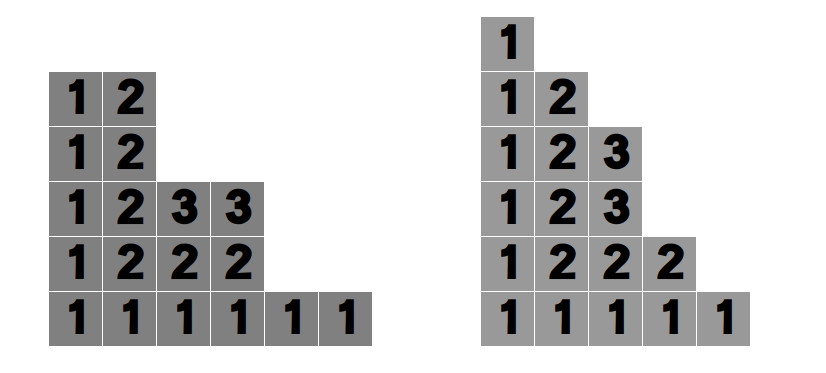
\includegraphics[scale=0.4]{picture/figure13.png}
	\end{figure}
	
	接下来将证明两个事实:减 Ferrers 棋盘进行翻转操作之后得到的是一个竖直型减 Ferrers 棋盘;翻转操作前后覆盖多项式不变。

	首先对第一个事实进行证明。
	
	\begin{lemma}
		棋盘 $S$ 是减 Ferrers 棋盘当且仅当对所有在棋盘中的格子 $(i,j)$ 编号 $\min(i,j)$ 后相同编号的格子构成一个 $L$ 形,且 $\forall p_i \neq 0 , p_i > p_{i+1},q_i > q_{i+1}$。
	\end{lemma}
	\begin{proof}
		对于存在某一个编号不构成 $L$ 形的棋盘,一定存在某行或某列不满足恰有一段前缀的格子属于 $S$,因此 $S$ 一定不是减 Ferrers 棋盘。
		
		考虑按照编号从大到小加入每一个 $L$ 形并维护每一列的高度,棋盘 $S$ 是减 Ferrers 棋盘当且仅当在这个过程中每一个编号的 $L$ 形加入后都得到减 Ferrers 棋盘。
		
		设仅考虑编号 $\geq i+1$ 的格子构成的棋盘为 $F(a_1,a_2\cdots,a_{q_{i+1}})$,加入编号为 $i$ 的 $L$ 形相当于将序列 $F$ 长度为 $q_i-1$ 的前缀加一,若序列 $F$ 长度不够则在后面补充 $0$,然后在序列最前面插入一个 $p_i$。此时同时满足以下两个条件是新棋盘是减 Ferrers 棋盘的充要条件:
		\begin{enumerate}
			\item $q_i > q_{i+1}$,若该条件不满足则第 $q_{i+1}$ 列将不满足恰有一段行前缀属于 $S$;
			\item $p_i > p_{i+1}$,若该条件不满足则序列 $F$ 不满足单调不增。
		\end{enumerate}
		即证明引理。
	\end{proof}
	
	\begin{theorem}
		对减 Ferrers 棋盘进行翻转操作后得到的棋盘一定是减 Ferrers 棋盘。
	\end{theorem}
	\begin{proof}
		由于减 Ferrers 棋盘编号后每个编号一定是 $L$ 形,因此只需要证明新的棋盘中 $p_i > p_{i+1},q_i > q_{i+1}$ 即可。由于初始棋盘满足该条件,因此若第 $i$ 个和第 $i+1$ 个 $L$ 形均翻转或不翻转,则条件显然成立。故仅需要考虑只有一个翻转的情况。
		
		不妨假设编号为 $i$ 的 $L$ 形不翻转,编号为 $i+1$ 的 $L$ 形翻转,另一种情况类似。设原棋盘中第 $i,i+1$ 个 $L$ 的左、下端长度为 $p_i,q_i,p_{i+1},q_{i+1}$,则 $p_i>q_i,p_{i+1}<q_{i+1}$。而 $p_i>q_i>q_{i+1},q_i>q_{i+1}>p_{i+1}$,因此这两个 $L$ 形仍然满足条件。
	\end{proof}
	
	与此同时由于翻转过后的棋盘满足 $p_i \geq q_i$,所以其是竖直型减 Ferrers 棋盘。
	
	然后对第二个事实进行证明。我们不证明事实本身,而证明容易推导出事实的结论。
	\begin{theorem}
		对于减 Ferrers 棋盘 $S$ 和其翻转得到的竖直型减 Ferrers 棋盘 $S'$,设集合 $P_S$ 表示 $G_S$ 中的所有简单有向链和简单环构成的集合,则存在一个双射 $$\phi:P_S \rightarrow P_{S'}$$ 使得若 $T \in P_S$,则
		\begin{enumerate}
			\item $\phi(T)$ 和 $T$ 覆盖相同的点集;
			\item $\phi(T)$ 是简单环当且仅当 $T$ 是简单环。
		\end{enumerate}
		
		一条简单有向链满足至少经过一个点且每个点至多经过一次,一个简单环满足至少经过一个点且环上每个点的入出度均为 $1$。
	\end{theorem}
	\begin{proof}
		考虑对 $v = \max_{p_i > 0} i$ 进行归纳。当 $v=0$ 时,两图都没有边,因此 $P$ 中仅有覆盖每个点的链,此时 $\phi(\{v\}) = \{v\}$ 满足条件。
		
		当结论对 $0$ 至 $v-1$ 均成立时,对于棋盘 $S,S'$,由于将编号为 $1$ 的格子删掉得到的两个棋盘 $S_1,S_1'$ 满足 $S_1'$ 是 $S_1$ 翻转得到的,因此存在一个双射 $\psi:P_{S_1} \rightarrow P_{S_1'}$ 满足题设条件。加入编号为 $1$ 的格子可看做在对应图上插入编号为 $1$ 的点,原编号为正的点编号加一,然后从 $1$ 向一段正整数的前缀连边,从另一段正整数的前缀向 $1$ 连边,自环不重复连接。
		
		对于 $T \in P_S$,若 $T \in P_{S_1}$ 则 $\phi(T) = \psi(T)$ 满足条件;若 $T = \{1\}$ 则 $\phi(T) = T$。否则考虑 $1$ 在 $T$ 中的情况以及 $S$ 变为 $S'$ 的过程中是否翻转编号为 $1$ 的 $L$ 形,$\phi(T)$ 的取值如下表:
		
		\begin{center}\begin{tabular}{|c|c|c|}
			\hline
			$T$ 的形态 & 未翻转时 $\phi(T) =$ & 翻转时 $\phi(T)=$ \\ \hline
			$R_1,1$ & $\psi(R_1) , 1$ & $1,\psi(R_1)$ \\ \hline
			$1,R_1$ & $1,\psi(R_1)$ & $\psi(R_1),1$ \\ \hline
			$1,R_1,1$ & $1,\psi(R_1),1$ & $1,\psi(R_1),1$ \\ \hline
			$R_1,1,R_2$ & $\psi(R_1),1,\psi(R_2)$ & $\psi(R_2),1,\psi(R_1)$ \\ \hline
		\end{tabular}\end{center}
		其中 $R_1,R_2$ 为 $P_{S_1}$ 中的某条简单有向链。用逗号将若干个路径或节点连接表示将它们拼接得到的简单有向链或简单环,其中情况三表示的是简单环,其余是简单有向链。
		
		容易验证 $\phi$ 的一对原像和像满足同时不是环或同时是环,且构成它们的点集是一致的,故只需要证明这样的连边不会导致某条边不属于 $S'$ 即可。
		
		对于 $R_1$ 或 $R_2$ 大小 $\leq 1$ 的情况,其在 $\psi$ 下的像为其本身。在 $L$ 形未翻转的情况下边没有发生改变,不会导致连边不存在;在 $L$ 形翻转的情况下边的方向也发生了翻转,其所对应的棋盘上的格子也做了翻转,因此该边也是存在的。
		
		对于 $R_1$ 或 $R_2$ 大小 $>1$ 的情况,可以利用减 Ferrers 棋盘的直接推论“从 $1$ 能直接到达以及能直接到达 $1$ 的集合总是其他点的对应集合的超集”论证。由于情况较多仅举一例:
		
		当 $T = 1,R_1$ 且编号为 $1$ 的 $L$ 形翻转时,设 $\psi(R_1)$ 的终止节点为 $w$ 且 $(w,1) \not\in G_{S'}$,即 $(1,w) \not\in G_S$,故 $G_S$ 中 $w$ 没有入度,则 $w$ 一定是 $R_1$ 的起始节点。而 $T = 1,R_1$ 意味着 $(1,w) \in G_S$ 产生矛盾,因此 $(w,1) \in G_{S'}$,这条路径是合法路径。
		
		对于其他情况可以类似证明。综合上面的讨论可以证明 $\phi$ 的合法性。
	\end{proof}

	综合上述两个事实,有
	\begin{theorem} \label{decrease=upright}
		对于任意减 Ferrers 棋盘,存在一个竖直型减 Ferrers 棋盘与其拥有相同的覆盖多项式。
	\end{theorem}

	构造出对应的竖直型减 Ferrers 棋盘后计算出其覆盖多项式即可得到原减 Ferrers 棋盘的覆盖多项式。
	
	该分解定理在轮廓线棋盘上使用会受到很大的限制,在参考文献 \cite{1997Factorization} 中进行了一定的讨论,但由于篇幅原因无法展现,感兴趣的读者可自行阅读。
	
	\section{总结}
	
	本文对组合数学中的棋盘模型进行了简单的介绍,通过对 Ferrers 棋盘的下降幂棋盘多项式的性质进行应用和推广得到了其在三种排列问题中的应用。
	
	然而本文所介绍的棋盘理论知识仅仅是当下棋盘理论研究成果的冰山一角,如:\cite{2001Rook} 中利用棋盘模型得到了与二分图完美匹配相关的若干结论;\cite{2014m} 中给出了定理 \ref{mxiajiangmi} 的 q-analogue 形式并利用其推导了拓展卡特兰数的若干性质;\cite{2004Rook} 则利用棋盘理论对 $p-q$ 斯特林数给出了组合解释。这些问题由于本文篇幅有限,且笔者能力有限没有找到它们在实际问题中的较好应用因而没有一一展开讨论。
	
	希望本文可以起到抛砖引玉的作用,让读者更好地认识棋盘理论,更好地感受棋盘理论在计数问题中的强大应用。期待有更多使用棋盘模型的问题在信息学竞赛中出现。
	
	\section{致谢}
	
	感谢中国计算机学会提供学习和交流的平台。
	
	感谢国家集训队教练高闻远的指导。
	
	感谢家人对我的陪伴与支持。
	
	感谢长郡中学谢秋锋老师的关心与指导。
	
	感谢叶闻捷学长、郭晓旭前辈给予我写作本文的启发。
	
	感谢长郡中学 2021 届信息组的同学给予我的帮助与陪伴。
	
	感谢高子翼同学、谢睿杰同学为本文验稿并提出建议。
	
	感谢其他给予我帮助的老师与同学。
	
	\bibliography{appendix}
\end{document}